%% GENERATED by build.py from manuscript.tex -- do not edit; edit manuscript.tex instead.
%% Reliability beyond accuracy in machine learning of magnetic materials
%% Springer Nature LaTeX template (sn-jnl.cls, Version 3.1 December 2024), Nature Portfolio reference style (sn-nature).
%% Follows the template user manual, section 2.2 (Nature Portfolio journals): no footnotes; references pasted into this
%% file (run  python inline_references.py  after changing citations or references.bib); Methods after the main text and the
%% reference list; tables, figures with their legends and Extended Data at the end of the file.
%% One .tex file (no \input); figure files sit next to this file (no subfolders).
%% Left out on purpose for now: author names and affiliations, and the Declarations (funding, competing interests, data,
%% code and materials availability, author contributions, use of large language models).
%% Peer-review copy (double-spaced, line numbers): change the class options to [referee,lineno,pdflatex,sn-nature].

\documentclass[referee,lineno,pdflatex,sn-nature]{sn-jnl}

\usepackage{graphicx}%
\usepackage{multirow}%
\usepackage{amsmath,amssymb,amsfonts}%
\usepackage{amsthm}%
\usepackage{mathrsfs}%
\usepackage[title]{appendix}%
\usepackage{xcolor}%
\usepackage{textcomp}%
\usepackage{manyfoot}%
\usepackage{booktabs}%

\newcommand{\muB}{\ensuremath{\mu_\mathrm{B}}}
\newcommand{\Tc}{\ensuremath{T_\mathrm{C}}}
\newcommand{\mcell}{\ensuremath{m_\mathrm{cell}}}
\newcommand{\mfu}{\ensuremath{m_\mathrm{fu}}}
\newcommand{\ci}[2]{[#1, #2]}
%% Table helpers: a header on two lines, and an estimate with its 95% interval on the line below.
\newcommand{\hd}[1]{\begin{tabular}[b]{@{}c@{}}#1\end{tabular}}
\newcommand{\hdl}[1]{\begin{tabular}[b]{@{}l@{}}#1\end{tabular}}
\newcommand{\est}[3]{\begin{tabular}[t]{@{}l@{}}#1\\{[}#2, #3{]}\end{tabular}}

\raggedbottom
\unnumbered
%% The class forbids a page break after any hyphenated line (\brokenpenalty 10000), which leaves pages several lines short.
\brokenpenalty=500

\begin{document}

\title[Reliability beyond accuracy in magnetic-materials ML]{Reliability beyond accuracy in machine learning of magnetic materials}

%% ---- AUTHORS AND AFFILIATIONS: left blank for now (fill in and remove the leading %% to activate) ----
%% \author*[1]{\fnm{} \sur{}}\email{}
%% \author[1]{\fnm{} \sur{}}
%% \affil*[1]{\orgdiv{}, \orgname{}, \orgaddress{\street{}, \city{}, \postcode{}, \country{}}}

\abstract{Machine learning models of magnetic materials, trained on computed and literature-mined databases, are usually judged by their accuracy on held-out data. Accuracy does not show that added physical descriptors carry information, that stated uncertainties can be trusted or that predictions hold for unfamiliar chemistry. We measured these properties separately, on one curated dataset of magnetic ordering, Curie temperature and computed magnetic moment. Descriptors from density functional theory gave no detectable gain over composition for ordering or the Curie temperature, although the design could detect only large effects, and a small gain for the computed moment mostly reflected cell size. Conformal intervals and prediction sets were calibrated on average but under-covered the highest predictions and the antiferromagnetic and ferrimagnetic classes unless the method was chosen with care. Ordering labels from computation and from experiment agreed no better than chance; neutron-determined structures matched the experimental labels but mostly not the computed ones, and models transferred poorly between the sources. On an audited external benchmark of experimental Curie temperatures, error grew with chemical distance from the training data, and performance in unseen chemical systems was much weaker, with wide uncertainty. Models for materials discovery should report descriptor gains, calibration and transfer alongside accuracy.}

\keywords{magnetic materials, machine learning, Curie temperature, magnetic ordering, uncertainty quantification, conformal prediction, distribution shift}

\maketitle

%% ===================================================================================================================
\section{Introduction}\label{sec:intro}

Magnetic materials underpin electric motors, generators and data storage\cite{gutfleisch2011magnetic,coey2010magnetism}, and three kinds of resource have made it possible to train machine-learning models of magnetism: high-throughput density functional theory (DFT) databases\cite{jain2013materials,saal2013oqmd,choudhary2020jarvis,curtarolo2012aflow}, databases mined from the literature\cite{kelly2025curie,court2020phase,itani2025nemad} and curated collections of magnetic structures\cite{gallego2016magndata}. Models that use only the chemical composition report errors of 56--69~K for the Curie temperature \Tc{} and accuracies of 78--91\% for magnetic ordering\cite{nelson2019curie,long2021ferro,belot2023curie,merker2022classifiers,itani2025nemad,abediorang2026curie}. Graph networks that read the crystal structure\cite{merker2022classifiers,choudhary2021alignn} and high-throughput DFT workflows\cite{horton2019ordering,frey2020oxides} offer other routes. These figures come from random or stratified splits of a single dataset (Supplementary Table~9). None of the studies that we examined tested on data grouped by chemistry or drawn from another label source, and in the one cross-dataset test that we found the \Tc{} error rose from 69 to 90~K\cite{belot2023curie}.

Accuracy on such splits is necessary, but work elsewhere in materials informatics shows that it is not sufficient. Random splits overstate the ability to extrapolate\cite{meredig2018extrapolation,xiong2020forwardcv,li2023critical,li2024mdhit,omee2024ood}, and standardised grouped splits are now available for testing it\cite{witman2025matfold}. Accuracy on a proxy target need not carry over to the task of interest\cite{bartel2020stability}. Uncertainty estimates need their own validation\cite{tran2020uq,varivoda2023uq,palmer2022calibration}, and leakage between training and test data inflates reported performance\cite{kapoor2023leakage,dunn2020matbench}. Methods exist for distribution shift\cite{koh2021wilds,tibshirani2019covariate} and for abstaining from uncertain predictions\cite{geifman2017selective}, and active learning depends on uncertainty that can be used\cite{lookman2019active}. For magnetic materials, however, no single study has measured descriptor gains, calibration and transfer on the same data and the same models, with resampling at the level at which the records are dependent.

We made these measurements for three targets: magnetic ordering, \Tc{} and the magnetic moment computed by DFT. We asked whether DFT descriptors add information beyond composition, whether uncertainties are calibrated overall and within subgroups, and whether predictions transfer to unfamiliar chemistry and to labels from another source. The answers differ from question to question, and none follows from the accuracy of the model. Several errors that we made and corrected in our own earlier analyses (Methods) show how easily each question is answered wrongly.

%% ===================================================================================================================
\section{Results}\label{sec:results}

\subsection{Curated data and baselines}\label{sec:dataset}

We merged nine files from seven providers into one schema that records the source of every row (507,828 rows; Methods): Materials Project\cite{jain2013materials}, OQMD\cite{saal2013oqmd}, JARVIS-DFT\cite{choudhary2020jarvis}, two NEMAD releases\cite{itani2025nemad}, the ChemDataExtractor Curie and N\'eel database\cite{kelly2025curie}, MAGNDATA\cite{gallego2016magndata} and two experimental literature compilations. Written curation rules, which only remove rows, defined each target (Table~\ref{tab:dataset}). Two removals were large. Five rules removed superconducting, ferroelectric and N\'eel temperatures and out-of-range values that had been recorded as Curie temperatures, which reduced the \Tc{} target from 34,322 to 29,740 records. All 15,493 JARVIS ordering labels were set aside, because every one read `ferromagnetic': the value was a default written by our data collector and not an assignment. The moment target is the total magnetic moment of the DFT cell at 0~K (\mcell{}); it is not an experimental saturation magnetization. Because \mcell{} grows with the number of atoms in the cell, we also analysed the moment per formula unit (\mfu{}).

The \Tc{} labels remain noisy after curation. In a screen of 200 randomly drawn records, judged from the title of the source paper, 11.0\% (95\% interval 7.4--16.1\%) were flagged as likely to be wrong; 12 of these 22 records came from the text-mined source, which supplied 61 of the 200. A further 16\% of the titles concerned a different compound, which a title alone cannot resolve, so the share of doubtful labels lies between 11\% and 27\% (Supplementary Table~5). Repeated records of one formula differ by a median standard deviation of 4.2~K, but for 13\% of such formulas the spread exceeds 100~K.

Predictors form three nested tiers. Tier~1 holds 65 descriptors computed from the composition alone. Tier~2 adds 8 descriptors of the oxidation states. Tier~3 adds 24 non-magnetic DFT properties of the most stable computed polymorph of each formula, such as the formation energy, band gap, symmetry, volume, density and elastic and dielectric constants (Methods), and is available for 28,512 materials. We kept the magnetic outputs of DFT out of Tier~3, because they are the source of the moment labels and of part of the ordering labels. Every split keeps all records of one reduced formula together.

Within the training distribution, composition alone was accurate. For ordering, XGBoost\cite{chen2016xgboost} reached a macro-averaged F1 score (macro-F1) of 0.727 (0.711--0.744), compared with 0.469 for multinomial logistic regression and 0.151 for the majority class. For \Tc{}, gradient boosting\cite{ke2017lightgbm,pedregosa2011sklearn} reached a mean absolute error (MAE) of 76.2~K (69.9--82.5~K) and a coefficient of determination $R^2$ of 0.78, compared with 147.2~K for ridge regression and 218.8~K for the training mean. For \mcell{}, gradient boosting reached 2.58~\muB{} per cell ($R^2$ 0.70). Other ordering scores in this paper come from other setups: 0.692 is the mean of Tier~1 XGBoost over ten splits (Supplementary Table~7), and 0.712 is the formula-grouped value in the leave-chemical-system-out comparison (ten random splits, fixed hyperparameters). Compounds that are trivially non-magnetic do not carry the ordering score: over ten splits, restricting the test set to compounds that contain an element capable of magnetism lowered macro-F1 only from 0.692 to 0.681. The weak classes are antiferromagnets and ferrimagnets, with recalls near 0.55 and 0.49 (Supplementary Table~7).

\subsection{Computed descriptors add little}\label{sec:rq1}

To test whether DFT descriptors add information, we compared the tiers on matched populations: the materials with complete Tier~3 descriptors, used with identical rows, splits, hyperparameter grids and metrics at every tier, over ten prespecified splits (Fig.~\ref{fig:rq1}, Extended Data Table~\ref{tab:ed_tiers}). We call a difference stable only if two intervals exclude zero, one that accounts for refitting\cite{nadeau2003inference} and one from a bootstrap over formulas, and if at least seven of the ten splits agree in sign; this is a reporting convention and not a hypothesis test. The nine contrasts between Tier~1 and Tier~3 (three targets by three algorithms) form the primary family and are Holm-corrected\cite{holm1979simple}.

For ordering and \Tc{}, no algorithm showed a stable effect of Tier~2 or Tier~3, and every primary adjusted $P$ value was 1.0. For \Tc{} the Tier~3 point estimates were losses: $-14.3$~K ($-42.5$ to $+13.9$) for gradient boosting, $-8.2$~K ($-48.3$ to $+32.0$) for XGBoost and $-14.4$~K ($-33.5$ to $+4.8$) for ridge regression with clipped inputs. This design detects only large effects, of 27--56~K for \Tc{} and 0.04--0.09 in macro-F1 for ordering, and the intervals leave room for \Tc{} gains of up to 5--32~K. We therefore report no detectable gain; we do not claim that a gain is absent. Pooling the three algorithms, which are scored on the same test rows, narrowed the \Tc{} interval: the mean Tier~3 change was $-12.3$~K ($-32.7$ to $+8.1$; worse in eight of ten splits), so the average algorithm gains less than 10~K, our margin of practical relevance, although the pooled contrast still detects only changes of 28~K or more. For ordering the pooled change was $-0.002$ ($-0.035$ to $+0.031$), which does not exclude the margin of 0.02 macro-F1. A larger hyperparameter search for gradient boosting (64 settings instead of 4, the same for both tiers) did not change the picture: the Tier~3 change was $-11.8$~K ($-35.2$ to $+11.7$), and the test errors of both tiers moved by less than 2~K (Tier~1 203.7~K and Tier~3 215.5~K, compared with 202.9 and 217.2~K), although the validation error of the selected settings was 27 and 34~K lower than that of the original grid, a gain that did not carry over to the test rows. The formula-bootstrap interval of the tuned contrast ended just below zero ($-21.9$ to $-0.04$) but the refit-aware interval did not, so we class it as a borderline loss and not as a gain. The matched \Tc{} population is also much harder than the full one (Tier~1 MAE 203~K, compared with 76~K), so the result applies to materials that have a full DFT record.

For \mcell{}, Tier~3 gave gains that were stable but small: $+0.079$~\muB{} per cell ($+0.030$ to $+0.127$) for gradient boosting and $+0.062$ ($+0.023$ to $+0.101$) for XGBoost, or 2--3\% of the MAE (adjusted $P=0.046$); pooled over the three algorithms the gain was $+0.065$~\muB{} per cell ($+0.038$ to $+0.092$), positive in all ten splits. A single number, the count of sites in the DFT cell, recovered about 70\% of the gradient-boosting gain when it was added to Tier~2, and what Tier~3 added beyond it was not resolved ($+0.024$; $-0.003$ to $+0.050$). The moment per formula unit behaved in the same way. Its gains were stable for all three algorithms ($+0.031$~\muB{} per formula unit for gradient boosting; $+0.014$ to $+0.048$), but beyond the site count they were not resolved for the two tree models, whereas ridge regression kept a stable $+0.030$ (Fig.~\ref{fig:rq1}d, Supplementary Table~8). Dividing the moment by the number of sites removes the cell size directly; a gain of 2.9\% of the MAE for gradient boosting, 2.8\% for XGBoost and 6.0\% for ridge regression then remained, and earlier analyses traced it mainly to other outputs of the same DFT calculation (Methods). The moment gain is therefore real but small, and for the per-cell and per-formula-unit targets it is mostly an effect of cell size. A site count can still help an intensive target because it is a weak proxy for the magnetic ordering: cells that hold more than one formula unit (42\% of the rows) have a lower moment per formula unit and more often an antiferromagnetic label (mean moment 3.1~\muB{} and 3\% antiferromagnetic labels for cells with one formula unit, 1.7~\muB{} and 17\% for cells with three or four; Supplementary Table~15), but the association is modest (Spearman $\rho=-0.16$ with the moment) and we did not test the mechanism further.

A null result may reflect the choice of descriptors, because Tier~3 contains no magnetic quantities. For \Tc{}, where the magnetic outputs of DFT cannot leak the label, we therefore added three further kinds of physics to the matched population (Extended Data Table~\ref{tab:ed_magphys}): ten descriptors of the magnetic sublattice computed from the crystal structure, including the metal--anion--metal angles that govern superexchange; four magnetic outputs of DFT; and a fixed 64-dimensional crystal embedding from the pretrained interatomic potential CHGNet\cite{deng2023chgnet}. None improved on composition alone. Against Tier~1 the estimates ranged from $-10.8$ to $+9.5$~K, and every interval included zero. Relative to Tier~3, the embedding gave $+19.2$~K for XGBoost, which was stable in a single realization, and the magnetic outputs gave a borderline $+19.6$~K for gradient boosting. Both roughly recover the loss incurred at Tier~3, and neither exceeds Tier~1.

Feature attribution did not reveal this. TreeSHAP\cite{lundberg2017shap,lundberg2020treeshap} assigned 40\% (ordering) and 36\% (\Tc{}) of the mean absolute attribution of the Tier~3 XGBoost models to DFT descriptors that did not improve accuracy. Correlated composition and DFT features can carry the same information, so attribution shows that a feature is used and not that it adds value.

\subsection{Average coverage hides failures}\label{sec:rq2}

We next asked whether the uncertainties can be trusted. For regression we compared three conformal methods\cite{vovk2005algorithmic,lei2018distribution,angelopoulos2023gentle}, which have been used for machine-learned interatomic potentials\cite{hu2022conformal} at a nominal coverage of 90\%: split conformal prediction, which gives intervals of constant width; normalized conformal prediction, which scales the width by a learned difficulty model\cite{papadopoulos2011normalized}; and conformalized quantile regression (CQR)\cite{romano2019cqr} (Fig.~\ref{fig:rq2}a,b, Extended Data Table~\ref{tab:ed_intervals}). On average all three met the nominal coverage, as the theory guarantees: 89.3\%, 90.3\% and 89.4\% for \Tc{}, and 90.0--90.1\% for \mcell{}.

The methods differed within subgroups, which we defined without reference to the difficulty score of any method. In the top decile of predicted \Tc{}, the normalized method covered 87.4\%, the constant-width method 65.5\% and quantile regression 68.6\%. For text-mined labels the figures were 86.0\% compared with 78--79\%, and for the highest predicted third of \mcell{} they were 86.7\% compared with 72.3\% and 83.4\%. The normalized method came closest to nominal coverage in these cases, but it was not best everywhere (Supplementary Table~11). On labels taken from computational papers it covered 86.6\%, compared with 90.4\% for the constant-width method; on several chemical families and on the two experimental compilations the other two methods covered more (92--97\% compared with 89--92\%), because their intervals are wide everywhere. The normalized method was the most stable: across splits its \Tc{} coverage had a standard deviation of 2.5 points, compared with about 6 points for the other two. Records of one formula are dependent, so about 4,200 calibration rows act like only 250--340 independent ones (Supplementary Table~6).

Coverage was not protected against shift. In the decile farthest from the training chemistry it was 86.6--89.7\%, and calibrating the normalized method separately for each distance quartile raised its coverage there from 88.2\% to 90.3\%. When intervals were calibrated on the larger experimental compilation and tested on text-mined rows (one frozen split), \Tc{} coverage was 76.9\% for the constant-width method, 80.3\% for quantile regression and 85.1\% for the normalized method.

The ordering classifier was trained with balanced class weights, so its raw probabilities follow a uniform prior. Correcting them to the training prior\cite{saerens2002adjusting} worsened the expected calibration error from 0.064 to 0.090, and adding temperature scaling\cite{guo2017calibration} reduced it to 0.014 (Extended Data Table~\ref{tab:ed_ordcal}). Marginal conformal prediction sets met the nominal coverage overall (89.8\%) by covering ferromagnets (96.2\%) and non-magnets (97.7\%) too often, and antiferromagnets (57.0\%) and ferrimagnets (54.3\%) too rarely (Fig.~\ref{fig:rq2}c). Class-conditional sets\cite{vovk2013conditional} covered 89.8--90.9\% of every class, at a mean set size of 1.61 classes compared with 1.39.

\subsection{Ordering labels depend on their source}\label{sec:provenance}

For 949 formulas, both Materials Project and an experimental source supply an ordering label. The two labels agreed for 28\% of these formulas, with Cohen's $\kappa=0.00$ ($-0.03$ to $0.03$), which is no better than chance. Of 508 antiferromagnets in the experimental sources, 336 (66\%) are ferromagnetic in Materials Project (Supplementary Table~12). This is what a high-throughput workflow produces when it starts from ferromagnetic configurations and enumerates antiferromagnetic orderings for only part of the database\cite{horton2019ordering}: in that survey, 31,631 of 33,986 magnetic entries (93\%) were in a ferromagnetic configuration, with only a few well-known antiferromagnets or ferrimagnets among them.

An independent reference shows which side is wrong. MAGNDATA\cite{gallego2016magndata,gallego2016magndata2}, hosted by the Bilbao Crystallographic Server\cite{aroyo2011bcs,aroyo2006bcs1,aroyo2006bcs2}, collects magnetic structures determined mainly by neutron diffraction; we labelled each ordered, collinear structure ferromagnetic, antiferromagnetic or ferrimagnetic from its own moments (840 compositions; Methods). The experimental labels agreed with these structures for 92\% of 442 shared compositions (95\% interval 90--95\%; $\kappa=0.72$), but the Materials Project labels for only 22\% of 251 (17--28\%; $\kappa=0.03$). Of 218 antiferromagnets, Materials Project called 125 (57\%) ferromagnetic and 30 non-magnetic. Where Materials Project and the experimental source disagreed on a composition that MAGNDATA also covers, the experimental label matched the structure in 107 of 114 cases (Supplementary Table~12c).

Models did not bridge this gap (Extended Data Table~\ref{tab:ed_general}). A model trained on Materials Project labels and tested on experimental labels reached a balanced accuracy of 0.337 (0.273--0.396). This cannot be distinguished from models trained on permuted labels (median 0.342) and is far below the 0.769 of a model trained on experimental labels; its recall for antiferromagnets was 7\%. The test compositions were no farther from the training compositions than within Materials Project itself (median distance to the nearest training formula 0.081, compared with 0.077), so in this direction the failure lies in the definition of the labels and not in the chemistry. In the reverse direction the balanced accuracy was 0.384 (0.366--0.401), just above the 97.5th percentile of the permuted-label models (0.351) and far below the within-source value of 0.591. Here the chemistry differs as well (median distance 0.169, compared with 0.033 within the experimental sources), so the two causes cannot be separated. A pooled ordering score therefore measures agreement with a labelling convention as much as the ability to predict magnetic order.

\subsection{Transfer to unfamiliar chemistry}\label{sec:rq3}

Within our data, holding out whole chemical systems (sets of elements) instead of formulas lowered the ordering macro-F1 from 0.712 to 0.684, a change of $-0.028$ ($-0.041$ to $-0.016$) that had the same sign in all ten paired splits and fell most heavily on ferrimagnets (Extended Data Table~\ref{tab:ed_general}). The moment error rose slightly but not stably ($+0.073$~\muB{} per cell; $-0.009$ to $+0.154$), and the change in \Tc{} error was not resolved ($+2.7$~K; $-16.8$ to $+22.2$).

For an external test we used a public table of 2,500 experimental Curie temperatures that was curated for an independent study\cite{malaei_magnetic_data,abediorang2026curie}. The table lists ferromagnets only, so it says nothing about ferrimagnets or about N\'eel temperatures. We scored the Tier~1 XGBoost model for \Tc{} and its normalized conformal intervals on this table without retraining or tuning. An audit came first (Methods; Supplementary Table~1). When compositions were compared, and not formula strings, 1,998 records (80\%) were already in our repository, and 1,200 (48\%) carried a value within 0.5~K of one that we held. On those records the model scored $R^2$ 0.90, which measures recall of training labels and not prediction. After 105 records were excluded for stated reasons, 2,395 remained, of which 465 were compositions that the model had never seen.

On these 465 blind records, from 81 clusters of source papers, the MAE was 102.7~K (75.1--143.6~K) and $R^2$ was 0.69 (0.43--0.82), and the intervals covered 89.5\% (Fig.~\ref{fig:rq3}, Extended Data Table~\ref{tab:ed_external}). Blind compositions in chemical systems that occur in the training data scored an MAE of 90.6~K and $R^2$ of 0.78. The 69 records in unseen chemical systems, from only 18 clusters, scored an MAE of 171.9~K (82.6--293.7~K) and $R^2$ of $-0.17$ ($-1.02$ to $0.64$). Performance in unseen systems is thus much weaker, with wide uncertainty: compared with blind records in seen systems, the $R^2$ difference was $-0.95$ ($-1.69$ to $-0.06$) and the MAE difference $+81$~K ($-27$ to $+165$; Supplementary Table~2). A rule that we fixed beforehand allows the statement `no skill beyond the mean' only if the upper limit of $R^2$ is at most 0.2, and that condition is not met; the upper limit is 0.21 even when chemical systems are the resampling unit (Supplementary Table~4). Skill in unseen chemical systems is therefore not established, and its absence is not established either.

Error followed a similarity measure that we fixed in advance, the composition distance to the nearest training formula. On the blind records, error rose with distance (Spearman's $\rho=0.28$; 0.10--0.49), and the MAE grew from 62~K in the closest quartile to 165~K in the farthest (Fig.~\ref{fig:distance}, Extended Data Fig.~\ref{fig:ed_scatter}). The normalized intervals widened, from 388 to 529~K, but not enough: coverage fell from 0.95 to 0.85 (Supplementary Table~3). Distance accounts for only part of the result for unseen systems, because blind records in seen systems at comparable distances kept an $R^2$ of 0.75.

\subsection{A first filter for screening}\label{sec:screening}

What do such predictions support in practice? On the 465 blind records, abstaining on the half of the compositions that lie farthest from the training data lowered the MAE from 103 to 71~K and brought coverage to 0.93 (Extended Data Table~\ref{tab:ed_screening}). Abstaining on the half with the widest intervals lowered the error by a similar amount (73~K) but left coverage at 0.88; the intervals of the two rules overlap, so we do not rank them. For a room-temperature screen (\Tc{} above 300~K; base rate 0.57), the point prediction had a recall of 0.94 and a precision of 0.77. Deciding only when the 90\% interval lay wholly above or wholly below 300~K settled 37\% of the records, with an accuracy of 92.5\%. The intervals are too wide to rank candidates within one family, but abstention and interval-based decisions make the model usable as a first filter.

The same rules behave differently inside the training chemistry (Extended Data Table~\ref{tab:ed_internal}; means over the ten internal test sets). Abstaining on the widest intervals was effective: keeping the narrowest half lowered the MAE from 103 to 43~K at a coverage of 0.92. Abstaining on composition distance was not: the closest half had an MAE of 86~K and the closest quarter 103~K, so distance helps on external data, which lie farther from the training chemistry, but not within it. For the room-temperature screen (base rate 0.45) the point prediction had a precision of 0.82 and a recall of 0.88, and deciding only when the 90\% interval excluded 300~K settled 44\% of the records with an accuracy of 97.6\%; precision among the 25 highest predictions was 0.96.

%% ===================================================================================================================
\section{Discussion}\label{sec:discussion}

The properties that we measured are related, but none can be inferred from another. Composition-only models were accurate, yet DFT descriptors gave no detectable gain while receiving more than a third of the attribution. The most accurate ordering model needed both prior correction and temperature scaling before its probabilities were calibrated, and its marginal prediction sets covered antiferromagnets and ferrimagnets little more than half the time. Intervals that were calibrated on average lost coverage with chemical distance and with a change of label source. A \Tc{} model with $R^2$ 0.78 inside the training distribution has no established skill in unseen chemical systems. An ordering model with macro-F1 0.73 transfers poorly between computed and experimental labels: at the level of permuted labels in one direction and barely above it in the other. Some of these outcomes were expected in principle, because marginal conformal guarantees do not extend to subgroups and balanced class weights distort probabilities. What we add is their size for magnetic materials, and evidence on which simple remedies work.

Why did DFT descriptors not help? We offer two explanations; the first has been tested only in part. First, the DFT values describe the lowest-energy computed polymorph of a formula, whereas a measured \Tc{} may belong to another structure, a doped sample or a film. Where the source reports a space group and it equals that of the computed polymorph (536 of the 4,602 matched records), Tier~3 still gave no gain ($-10.9$~K, $-23.8$ to $+2.0$, pooled over the three algorithms; Supplementary Table~16), and the result did not differ detectably from that for records with another space group ($-4.9$~K; $-28.0$ to $+18.2$). The models were trained on all rows, however, and only 18\% of the records report a space group, so a harmful join is not excluded. The Tier~3 point estimates for \Tc{} were losses, and they did not shrink where the join was right, so this test does not support a noisy join as their cause. Second, composition already fixes much of what the scalar descriptors encode, and where a gain did appear it traced back largely to cell size. The null result is therefore narrow. It concerns descriptors joined by formula and used by tabular tree and linear models, together with one fixed embedding. It is not evidence against models that learn the coupling between structure and property end to end from the measured phase.

The study has limits. The external benchmark overlaps heavily with our sources, and the conclusion for unseen systems rests on 69 records from 18 clusters of papers. The label-noise screen was made from titles with the help of a language model, so its figures are estimates and not verified error rates. Formula-grouped splits are not perfectly disjoint: formulas written in two ways affect 0.6\% of the \Tc{} test rows and 1.3\% of the ordering test rows. The structural reference for the ordering labels covers only ordered, collinear structures that have been studied by diffraction (840 compositions, 251 of them with Materials Project labels), and the experimental sources draw on the same literature. The magnetic-physics test covers \Tc{} only, the larger tuning check covers gradient boosting and \Tc{} only, several comparisons rest on a single XGBoost realization, and we did not test end-to-end graph networks (Methods).

Several practices follow for evaluation. Descriptor sets should be compared on identical rows and repeated grouped splits, with an interval that accounts for refitting and a simple control for size. Coverage should be reported for subgroups that are defined independently of the uncertainty method. Novelty should be defined by composition and chemical system, and the values of an external test set should be checked against the training labels. Resampling should follow the dependence between records. Data collectors should be audited for default values, and labels for agreement across sources. For deployment, our results favour normalized or class-conditional conformal prediction, abstention on wide intervals (and, for chemistry far from the training data, on composition distance) and recalibration when the label source changes. In discovery the candidates are unfamiliar by definition. A model for discovery should therefore be judged by how it behaves away from its training data and by whether its uncertainty supports a decision, and not by accuracy within the training distribution alone.

%% ===================================================================================================================
%% References (one list, numbered in order of first citation; the Methods-only references are the last ones).
%% Generated from references.bib by inline_references.py -- do not edit between the markers by hand.
%%% BEGIN REFERENCES
\begin{thebibliography}{10}
\expandafter\ifx\csname url\endcsname\relax
  \def\url#1{\burl{#1}}\fi
\expandafter\ifx\csname urlprefix\endcsname\relax\def\urlprefix{URL }\fi
\providecommand{\bibinfo}[2]{#2}
\providecommand{\eprint}[2][]{\url{#2}}
\providecommand{\doi}[1]{\url{https://doi.org/#1}}
\bibcommenthead

\bibitem{gutfleisch2011magnetic}
\bibinfo{author}{Gutfleisch, O.} \emph{et~al.}
\newblock \bibinfo{title}{Magnetic materials and devices for the 21st century:
  stronger, lighter, and more energy efficient}.
\newblock \emph{\bibinfo{journal}{Advanced Materials}}
  \textbf{\bibinfo{volume}{23}}, \bibinfo{pages}{821--842}
  (\bibinfo{year}{2011}).

\bibitem{coey2010magnetism}
\bibinfo{author}{Coey, J. M.~D.}
\newblock \emph{\bibinfo{title}{Magnetism and Magnetic Materials}}
  (\bibinfo{publisher}{Cambridge University Press},
  \bibinfo{address}{Cambridge}, \bibinfo{year}{2010}).

\bibitem{jain2013materials}
\bibinfo{author}{Jain, A.} \emph{et~al.}
\newblock \bibinfo{title}{Commentary: The {Materials Project}: A materials
  genome approach to accelerating materials innovation}.
\newblock \emph{\bibinfo{journal}{APL Materials}} \textbf{\bibinfo{volume}{1}},
  \bibinfo{pages}{011002} (\bibinfo{year}{2013}).

\bibitem{saal2013oqmd}
\bibinfo{author}{Saal, J.~E.}, \bibinfo{author}{Kirklin, S.},
  \bibinfo{author}{Aykol, M.}, \bibinfo{author}{Meredig, B.} \&
  \bibinfo{author}{Wolverton, C.}
\newblock \bibinfo{title}{Materials design and discovery with high-throughput
  density functional theory: the {Open Quantum Materials Database (OQMD)}}.
\newblock \emph{\bibinfo{journal}{JOM}} \textbf{\bibinfo{volume}{65}},
  \bibinfo{pages}{1501--1509} (\bibinfo{year}{2013}).

\bibitem{choudhary2020jarvis}
\bibinfo{author}{Choudhary, K.} \emph{et~al.}
\newblock \bibinfo{title}{The joint automated repository for various integrated
  simulations ({JARVIS}) for data-driven materials design}.
\newblock \emph{\bibinfo{journal}{npj Computational Materials}}
  \textbf{\bibinfo{volume}{6}}, \bibinfo{pages}{173} (\bibinfo{year}{2020}).

\bibitem{curtarolo2012aflow}
\bibinfo{author}{Curtarolo, S.} \emph{et~al.}
\newblock \bibinfo{title}{{AFLOW}: An automatic framework for high-throughput
  materials discovery}.
\newblock \emph{\bibinfo{journal}{Computational Materials Science}}
  \textbf{\bibinfo{volume}{58}}, \bibinfo{pages}{218--226}
  (\bibinfo{year}{2012}).

\bibitem{kelly2025curie}
\bibinfo{author}{Kelly, C.~R.} \& \bibinfo{author}{Cole, J.~M.}
\newblock \bibinfo{title}{A dataset of {Curie} and {N{\'e}el} temperatures
  auto-generated with {ChemDataExtractor} and the {Snowball} algorithm}.
\newblock \emph{\bibinfo{journal}{Scientific Data}}
  \textbf{\bibinfo{volume}{12}}, \bibinfo{pages}{2000} (\bibinfo{year}{2025}).

\bibitem{court2020phase}
\bibinfo{author}{Court, C.~J.} \& \bibinfo{author}{Cole, J.~M.}
\newblock \bibinfo{title}{{Magnetic and superconducting phase diagrams and
  transition temperatures predicted using text mining and machine learning}}.
\newblock \emph{\bibinfo{journal}{npj Computational Materials}}
  \textbf{\bibinfo{volume}{6}}, \bibinfo{pages}{18} (\bibinfo{year}{2020}).

\bibitem{itani2025nemad}
\bibinfo{author}{Itani, S.}, \bibinfo{author}{Zhang, Y.} \&
  \bibinfo{author}{Zang, J.}
\newblock \bibinfo{title}{The northeast materials database for magnetic
  materials}.
\newblock \emph{\bibinfo{journal}{Nature Communications}}
  \textbf{\bibinfo{volume}{16}}, \bibinfo{pages}{9415} (\bibinfo{year}{2025}).

\bibitem{gallego2016magndata}
\bibinfo{author}{Gallego, S.~V.} \emph{et~al.}
\newblock \bibinfo{title}{{MAGNDATA}: towards a database of magnetic
  structures. {I}. {The} commensurate case}.
\newblock \emph{\bibinfo{journal}{Journal of Applied Crystallography}}
  \textbf{\bibinfo{volume}{49}}, \bibinfo{pages}{1750--1776}
  (\bibinfo{year}{2016}).

\bibitem{nelson2019curie}
\bibinfo{author}{Nelson, J.} \& \bibinfo{author}{Sanvito, S.}
\newblock \bibinfo{title}{Predicting the {Curie} temperature of ferromagnets
  using machine learning}.
\newblock \emph{\bibinfo{journal}{Physical Review Materials}}
  \textbf{\bibinfo{volume}{3}}, \bibinfo{pages}{104405} (\bibinfo{year}{2019}).

\bibitem{long2021ferro}
\bibinfo{author}{Long, T.}, \bibinfo{author}{Fortunato, N.~M.},
  \bibinfo{author}{Zhang, Y.}, \bibinfo{author}{Gutfleisch, O.} \&
  \bibinfo{author}{Zhang, H.}
\newblock \bibinfo{title}{{An accelerating approach of designing ferromagnetic
  materials via machine learning modeling of magnetic ground state and Curie
  temperature}}.
\newblock \emph{\bibinfo{journal}{Materials Research Letters}}
  \textbf{\bibinfo{volume}{9}}, \bibinfo{pages}{169--174}
  (\bibinfo{year}{2021}).

\bibitem{belot2023curie}
\bibinfo{author}{Belot, J.~F.}, \bibinfo{author}{Taufour, V.},
  \bibinfo{author}{Sanvito, S.} \& \bibinfo{author}{Hart, G. L.~W.}
\newblock \bibinfo{title}{Machine learning predictions of
  high-{Curie}-temperature materials}.
\newblock \emph{\bibinfo{journal}{Applied Physics Letters}}
  \textbf{\bibinfo{volume}{123}}, \bibinfo{pages}{042405}
  (\bibinfo{year}{2023}).

\bibitem{merker2022classifiers}
\bibinfo{author}{Merker, H.~A.} \emph{et~al.}
\newblock \bibinfo{title}{{Machine learning magnetism classifiers from atomic
  coordinates}}.
\newblock \emph{\bibinfo{journal}{iScience}} \textbf{\bibinfo{volume}{25}},
  \bibinfo{pages}{105192} (\bibinfo{year}{2022}).

\bibitem{abediorang2026curie}
\bibinfo{author}{Orang, A.~A.}, \bibinfo{author}{Alaei, M.} \&
  \bibinfo{author}{Oganov, A.~R.}
\newblock \bibinfo{title}{Predicting the {Curie} temperature of magnetic
  materials with machine learning: Descriptor engineering, graph neural
  networks, and the role of curated data}.
\newblock \emph{\bibinfo{journal}{Computational Materials Science}}
  \textbf{\bibinfo{volume}{269}}, \bibinfo{pages}{114663}
  (\bibinfo{year}{2026}).

\bibitem{choudhary2021alignn}
\bibinfo{author}{Choudhary, K.} \& \bibinfo{author}{DeCost, B.}
\newblock \bibinfo{title}{{Atomistic Line Graph Neural Network for improved
  materials property predictions}}.
\newblock \emph{\bibinfo{journal}{npj Computational Materials}}
  \textbf{\bibinfo{volume}{7}}, \bibinfo{pages}{185} (\bibinfo{year}{2021}).

\bibitem{horton2019ordering}
\bibinfo{author}{Horton, M.~K.}, \bibinfo{author}{Montoya, J.~H.},
  \bibinfo{author}{Liu, M.} \& \bibinfo{author}{Persson, K.~A.}
\newblock \bibinfo{title}{High-throughput prediction of the ground-state
  collinear magnetic order of inorganic materials using density functional
  theory}.
\newblock \emph{\bibinfo{journal}{npj Computational Materials}}
  \textbf{\bibinfo{volume}{5}}, \bibinfo{pages}{64} (\bibinfo{year}{2019}).

\bibitem{frey2020oxides}
\bibinfo{author}{Frey, N.~C.} \emph{et~al.}
\newblock \bibinfo{title}{High-throughput search for magnetic and topological
  order in transition metal oxides}.
\newblock \emph{\bibinfo{journal}{Science Advances}}
  \textbf{\bibinfo{volume}{6}}, \bibinfo{pages}{eabd1076}
  (\bibinfo{year}{2020}).

\bibitem{meredig2018extrapolation}
\bibinfo{author}{Meredig, B.} \emph{et~al.}
\newblock \bibinfo{title}{Can machine learning identify the next
  high-temperature superconductor? {Examining} extrapolation performance for
  materials discovery}.
\newblock \emph{\bibinfo{journal}{Molecular Systems Design \& Engineering}}
  \textbf{\bibinfo{volume}{3}}, \bibinfo{pages}{819--825}
  (\bibinfo{year}{2018}).

\bibitem{xiong2020forwardcv}
\bibinfo{author}{Xiong, Z.} \emph{et~al.}
\newblock \bibinfo{title}{{Evaluating explorative prediction power of machine
  learning algorithms for materials discovery using $k$-fold forward
  cross-validation}}.
\newblock \emph{\bibinfo{journal}{Computational Materials Science}}
  \textbf{\bibinfo{volume}{171}}, \bibinfo{pages}{109203}
  (\bibinfo{year}{2020}).

\bibitem{li2023critical}
\bibinfo{author}{Li, K.}, \bibinfo{author}{DeCost, B.},
  \bibinfo{author}{Choudhary, K.}, \bibinfo{author}{Greenwood, M.} \&
  \bibinfo{author}{Hattrick-Simpers, J.}
\newblock \bibinfo{title}{A critical examination of robustness and
  generalizability of machine learning prediction of materials properties}.
\newblock \emph{\bibinfo{journal}{npj Computational Materials}}
  \textbf{\bibinfo{volume}{9}}, \bibinfo{pages}{55} (\bibinfo{year}{2023}).

\bibitem{li2024mdhit}
\bibinfo{author}{Li, Q.}, \bibinfo{author}{Fu, N.}, \bibinfo{author}{Omee,
  S.~S.} \& \bibinfo{author}{Hu, J.}
\newblock \bibinfo{title}{{MD-HIT: Machine learning for material property
  prediction with dataset redundancy control}}.
\newblock \emph{\bibinfo{journal}{npj Computational Materials}}
  \textbf{\bibinfo{volume}{10}}, \bibinfo{pages}{245} (\bibinfo{year}{2024}).

\bibitem{omee2024ood}
\bibinfo{author}{Omee, S.~S.}, \bibinfo{author}{Fu, N.}, \bibinfo{author}{Dong,
  R.}, \bibinfo{author}{Hu, M.} \& \bibinfo{author}{Hu, J.}
\newblock \bibinfo{title}{{Structure-based out-of-distribution (OOD) materials
  property prediction: a benchmark study}}.
\newblock \emph{\bibinfo{journal}{npj Computational Materials}}
  \textbf{\bibinfo{volume}{10}}, \bibinfo{pages}{144} (\bibinfo{year}{2024}).

\bibitem{witman2025matfold}
\bibinfo{author}{Witman, M.~D.} \& \bibinfo{author}{Schindler, P.}
\newblock \bibinfo{title}{{MatFold: systematic insights into materials
  discovery models' performance through standardized cross-validation
  protocols}}.
\newblock \emph{\bibinfo{journal}{Digital Discovery}}
  \textbf{\bibinfo{volume}{4}}, \bibinfo{pages}{625--635}
  (\bibinfo{year}{2025}).

\bibitem{bartel2020stability}
\bibinfo{author}{Bartel, C.~J.} \emph{et~al.}
\newblock \bibinfo{title}{{A critical examination of compound stability
  predictions from machine-learned formation energies}}.
\newblock \emph{\bibinfo{journal}{npj Computational Materials}}
  \textbf{\bibinfo{volume}{6}}, \bibinfo{pages}{97} (\bibinfo{year}{2020}).

\bibitem{tran2020uq}
\bibinfo{author}{Tran, K.} \emph{et~al.}
\newblock \bibinfo{title}{Methods for comparing uncertainty quantifications for
  material property predictions}.
\newblock \emph{\bibinfo{journal}{Machine Learning: Science and Technology}}
  \textbf{\bibinfo{volume}{1}}, \bibinfo{pages}{025006} (\bibinfo{year}{2020}).

\bibitem{varivoda2023uq}
\bibinfo{author}{Varivoda, D.}, \bibinfo{author}{Dong, R.},
  \bibinfo{author}{Omee, S.~S.} \& \bibinfo{author}{Hu, J.}
\newblock \bibinfo{title}{{Materials property prediction with uncertainty
  quantification: A benchmark study}}.
\newblock \emph{\bibinfo{journal}{Applied Physics Reviews}}
  \textbf{\bibinfo{volume}{10}}, \bibinfo{pages}{021409}
  (\bibinfo{year}{2023}).

\bibitem{palmer2022calibration}
\bibinfo{author}{Palmer, G.} \emph{et~al.}
\newblock \bibinfo{title}{{Calibration after bootstrap for accurate uncertainty
  quantification in regression models}}.
\newblock \emph{\bibinfo{journal}{npj Computational Materials}}
  \textbf{\bibinfo{volume}{8}}, \bibinfo{pages}{115} (\bibinfo{year}{2022}).

\bibitem{kapoor2023leakage}
\bibinfo{author}{Kapoor, S.} \& \bibinfo{author}{Narayanan, A.}
\newblock \bibinfo{title}{Leakage and the reproducibility crisis in
  machine-learning-based science}.
\newblock \emph{\bibinfo{journal}{Patterns}} \textbf{\bibinfo{volume}{4}},
  \bibinfo{pages}{100804} (\bibinfo{year}{2023}).

\bibitem{dunn2020matbench}
\bibinfo{author}{Dunn, A.}, \bibinfo{author}{Wang, Q.},
  \bibinfo{author}{Ganose, A.}, \bibinfo{author}{Dopp, D.} \&
  \bibinfo{author}{Jain, A.}
\newblock \bibinfo{title}{Benchmarking materials property prediction methods:
  the {Matbench} test set and {Automatminer} reference algorithm}.
\newblock \emph{\bibinfo{journal}{npj Computational Materials}}
  \textbf{\bibinfo{volume}{6}}, \bibinfo{pages}{138} (\bibinfo{year}{2020}).

\bibitem{koh2021wilds}
\bibinfo{author}{Koh, P.~W.} \emph{et~al.}
\newblock \bibinfo{title}{{WILDS: A Benchmark of in-the-Wild Distribution
  Shifts}}.
\newblock \emph{\bibinfo{journal}{Proceedings of the 38th International
  Conference on Machine Learning}} \textbf{\bibinfo{volume}{139}},
  \bibinfo{pages}{5637--5664} (\bibinfo{year}{2021}).

\bibitem{tibshirani2019covariate}
\bibinfo{author}{Tibshirani, R.~J.}, \bibinfo{author}{{Foygel Barber}, R.},
  \bibinfo{author}{Cand{\`e}s, E.~J.} \& \bibinfo{author}{Ramdas, A.}
\newblock \bibinfo{title}{{Conformal Prediction Under Covariate Shift}}.
\newblock \emph{\bibinfo{journal}{Advances in Neural Information Processing
  Systems}} \textbf{\bibinfo{volume}{32}} (\bibinfo{year}{2019}).

\bibitem{geifman2017selective}
\bibinfo{author}{Geifman, Y.} \& \bibinfo{author}{El-Yaniv, R.}
\newblock \bibinfo{title}{{Selective Classification for Deep Neural Networks}}.
\newblock \emph{\bibinfo{journal}{Advances in Neural Information Processing
  Systems}} \textbf{\bibinfo{volume}{30}} (\bibinfo{year}{2017}).

\bibitem{lookman2019active}
\bibinfo{author}{Lookman, T.}, \bibinfo{author}{Balachandran, P.~V.},
  \bibinfo{author}{Xue, D.} \& \bibinfo{author}{Yuan, R.}
\newblock \bibinfo{title}{{Active learning in materials science with emphasis
  on adaptive sampling using uncertainties for targeted design}}.
\newblock \emph{\bibinfo{journal}{npj Computational Materials}}
  \textbf{\bibinfo{volume}{5}}, \bibinfo{pages}{21} (\bibinfo{year}{2019}).

\bibitem{chen2016xgboost}
\bibinfo{author}{Chen, T.} \& \bibinfo{author}{Guestrin, C.}
\newblock \bibinfo{title}{{XGBoost}: A scalable tree boosting system}.
\newblock \emph{\bibinfo{journal}{Proceedings of the 22nd ACM SIGKDD
  International Conference on Knowledge Discovery and Data Mining}}
  \bibinfo{pages}{785--794} (\bibinfo{year}{2016}).

\bibitem{ke2017lightgbm}
\bibinfo{author}{Ke, G.} \emph{et~al.}
\newblock \bibinfo{title}{{LightGBM}: A highly efficient gradient boosting
  decision tree}.
\newblock \emph{\bibinfo{journal}{Advances in Neural Information Processing
  Systems}} \textbf{\bibinfo{volume}{30}} (\bibinfo{year}{2017}).

\bibitem{pedregosa2011sklearn}
\bibinfo{author}{Pedregosa, F.} \emph{et~al.}
\newblock \bibinfo{title}{Scikit-learn: Machine learning in {Python}}.
\newblock \emph{\bibinfo{journal}{Journal of Machine Learning Research}}
  \textbf{\bibinfo{volume}{12}}, \bibinfo{pages}{2825--2830}
  (\bibinfo{year}{2011}).

\bibitem{nadeau2003inference}
\bibinfo{author}{Nadeau, C.} \& \bibinfo{author}{Bengio, Y.}
\newblock \bibinfo{title}{{Inference for the Generalization Error}}.
\newblock \emph{\bibinfo{journal}{Machine Learning}}
  \textbf{\bibinfo{volume}{52}}, \bibinfo{pages}{239--281}
  (\bibinfo{year}{2003}).

\bibitem{holm1979simple}
\bibinfo{author}{Holm, S.}
\newblock \bibinfo{title}{{A Simple Sequentially Rejective Multiple Test
  Procedure}}.
\newblock \emph{\bibinfo{journal}{Scandinavian Journal of Statistics}}
  \textbf{\bibinfo{volume}{6}}, \bibinfo{pages}{65--70} (\bibinfo{year}{1979}).

\bibitem{deng2023chgnet}
\bibinfo{author}{Deng, B.} \emph{et~al.}
\newblock \bibinfo{title}{{CHGNet} as a pretrained universal neural network
  potential for charge-informed atomistic modelling}.
\newblock \emph{\bibinfo{journal}{Nature Machine Intelligence}}
  \textbf{\bibinfo{volume}{5}}, \bibinfo{pages}{1031--1041}
  (\bibinfo{year}{2023}).

\bibitem{lundberg2017shap}
\bibinfo{author}{Lundberg, S.~M.} \& \bibinfo{author}{Lee, S.-I.}
\newblock \bibinfo{title}{A unified approach to interpreting model
  predictions}.
\newblock \emph{\bibinfo{journal}{Advances in Neural Information Processing
  Systems}} \textbf{\bibinfo{volume}{30}} (\bibinfo{year}{2017}).

\bibitem{lundberg2020treeshap}
\bibinfo{author}{Lundberg, S.~M.} \emph{et~al.}
\newblock \bibinfo{title}{From local explanations to global understanding with
  explainable {AI} for trees}.
\newblock \emph{\bibinfo{journal}{Nature Machine Intelligence}}
  \textbf{\bibinfo{volume}{2}}, \bibinfo{pages}{56--67} (\bibinfo{year}{2020}).

\bibitem{vovk2005algorithmic}
\bibinfo{author}{Vovk, V.}, \bibinfo{author}{Gammerman, A.} \&
  \bibinfo{author}{Shafer, G.}
\newblock \emph{\bibinfo{title}{Algorithmic Learning in a Random World}}
  (\bibinfo{publisher}{Springer}, \bibinfo{address}{New York},
  \bibinfo{year}{2005}).

\bibitem{lei2018distribution}
\bibinfo{author}{Lei, J.}, \bibinfo{author}{G'Sell, M.},
  \bibinfo{author}{Rinaldo, A.}, \bibinfo{author}{Tibshirani, R.~J.} \&
  \bibinfo{author}{Wasserman, L.}
\newblock \bibinfo{title}{Distribution-free predictive inference for
  regression}.
\newblock \emph{\bibinfo{journal}{Journal of the American Statistical
  Association}} \textbf{\bibinfo{volume}{113}}, \bibinfo{pages}{1094--1111}
  (\bibinfo{year}{2018}).

\bibitem{angelopoulos2023gentle}
\bibinfo{author}{Angelopoulos, A.~N.} \& \bibinfo{author}{Bates, S.}
\newblock \bibinfo{title}{Conformal prediction: A gentle introduction}.
\newblock \emph{\bibinfo{journal}{Foundations and Trends in Machine Learning}}
  \textbf{\bibinfo{volume}{16}}, \bibinfo{pages}{494--591}
  (\bibinfo{year}{2023}).

\bibitem{hu2022conformal}
\bibinfo{author}{Hu, Y.}, \bibinfo{author}{Musielewicz, J.},
  \bibinfo{author}{Ulissi, Z.~W.} \& \bibinfo{author}{Medford, A.~J.}
\newblock \bibinfo{title}{{Robust and scalable uncertainty estimation with
  conformal prediction for machine-learned interatomic potentials}}.
\newblock \emph{\bibinfo{journal}{Machine Learning: Science and Technology}}
  \textbf{\bibinfo{volume}{3}}, \bibinfo{pages}{045028} (\bibinfo{year}{2022}).

\bibitem{papadopoulos2011normalized}
\bibinfo{author}{Papadopoulos, H.}, \bibinfo{author}{Vovk, V.} \&
  \bibinfo{author}{Gammerman, A.}
\newblock \bibinfo{title}{Regression conformal prediction with nearest
  neighbours}.
\newblock \emph{\bibinfo{journal}{Journal of Artificial Intelligence Research}}
  \textbf{\bibinfo{volume}{40}}, \bibinfo{pages}{815--840}
  (\bibinfo{year}{2011}).

\bibitem{romano2019cqr}
\bibinfo{author}{Romano, Y.}, \bibinfo{author}{Patterson, E.} \&
  \bibinfo{author}{Cand{\`e}s, E.}
\newblock \bibinfo{title}{Conformalized quantile regression}.
\newblock \emph{\bibinfo{journal}{Advances in Neural Information Processing
  Systems}} \textbf{\bibinfo{volume}{32}} (\bibinfo{year}{2019}).

\bibitem{saerens2002adjusting}
\bibinfo{author}{Saerens, M.}, \bibinfo{author}{Latinne, P.} \&
  \bibinfo{author}{Decaestecker, C.}
\newblock \bibinfo{title}{Adjusting the outputs of a classifier to new a priori
  probabilities: a simple procedure}.
\newblock \emph{\bibinfo{journal}{Neural Computation}}
  \textbf{\bibinfo{volume}{14}}, \bibinfo{pages}{21--41}
  (\bibinfo{year}{2002}).

\bibitem{guo2017calibration}
\bibinfo{author}{Guo, C.}, \bibinfo{author}{Pleiss, G.}, \bibinfo{author}{Sun,
  Y.} \& \bibinfo{author}{Weinberger, K.~Q.}
\newblock \bibinfo{title}{On calibration of modern neural networks}.
\newblock \emph{\bibinfo{journal}{Proceedings of the 34th International
  Conference on Machine Learning}} \textbf{\bibinfo{volume}{70}},
  \bibinfo{pages}{1321--1330} (\bibinfo{year}{2017}).

\bibitem{vovk2013conditional}
\bibinfo{author}{Vovk, V.}
\newblock \bibinfo{title}{Conditional validity of inductive conformal
  predictors}.
\newblock \emph{\bibinfo{journal}{Machine Learning}}
  \textbf{\bibinfo{volume}{92}}, \bibinfo{pages}{349--376}
  (\bibinfo{year}{2013}).

\bibitem{gallego2016magndata2}
\bibinfo{author}{Gallego, S.~V.} \emph{et~al.}
\newblock \bibinfo{title}{{MAGNDATA}: towards a database of magnetic
  structures. {II}. {The} incommensurate case}.
\newblock \emph{\bibinfo{journal}{Journal of Applied Crystallography}}
  \textbf{\bibinfo{volume}{49}}, \bibinfo{pages}{1941--1956}
  (\bibinfo{year}{2016}).

\bibitem{aroyo2011bcs}
\bibinfo{author}{Aroyo, M.~I.} \emph{et~al.}
\newblock \bibinfo{title}{Crystallography online: {Bilbao Crystallographic
  Server}}.
\newblock \emph{\bibinfo{journal}{Bulgarian Chemical Communications}}
  \textbf{\bibinfo{volume}{43}}, \bibinfo{pages}{183--197}
  (\bibinfo{year}{2011}).

\bibitem{aroyo2006bcs1}
\bibinfo{author}{Aroyo, M.~I.} \emph{et~al.}
\newblock \bibinfo{title}{{Bilbao Crystallographic Server}: {I}. {Databases}
  and crystallographic computing programs}.
\newblock \emph{\bibinfo{journal}{Zeitschrift f{\"u}r Kristallographie}}
  \textbf{\bibinfo{volume}{221}}, \bibinfo{pages}{15--27}
  (\bibinfo{year}{2006}).

\bibitem{aroyo2006bcs2}
\bibinfo{author}{Aroyo, M.~I.}, \bibinfo{author}{Kirov, A.},
  \bibinfo{author}{Capillas, C.}, \bibinfo{author}{Perez-Mato, J.~M.} \&
  \bibinfo{author}{Wondratschek, H.}
\newblock \bibinfo{title}{{Bilbao Crystallographic Server}. {II}.
  {Representations} of crystallographic point groups and space groups}.
\newblock \emph{\bibinfo{journal}{Acta Crystallographica Section A}}
  \textbf{\bibinfo{volume}{62}}, \bibinfo{pages}{115--128}
  (\bibinfo{year}{2006}).

\bibitem{malaei_magnetic_data}
\bibinfo{author}{Orang, A.~A.} \& \bibinfo{author}{Alaei, M.}
\newblock \bibinfo{title}{Magnetic\_data: {Curie} temperatures of 2,500
  ferromagnetic compounds with source {DOIs} ({FM} folder)}.
\newblock \bibinfo{howpublished}{GitHub repository
  \url{https://github.com/malaei/Magnetic_data}} (\bibinfo{year}{2026}).
\newblock \bibinfo{note}{Version analysed: commit 1656315 (3 February 2026);
  accessed October 2026}.

\bibitem{kirklin2015oqmd}
\bibinfo{author}{Kirklin, S.} \emph{et~al.}
\newblock \bibinfo{title}{The {Open Quantum Materials Database (OQMD)}:
  assessing the accuracy of {DFT} formation energies}.
\newblock \emph{\bibinfo{journal}{npj Computational Materials}}
  \textbf{\bibinfo{volume}{1}}, \bibinfo{pages}{15010} (\bibinfo{year}{2015}).

\bibitem{ong2013pymatgen}
\bibinfo{author}{Ong, S.~P.} \emph{et~al.}
\newblock \bibinfo{title}{Python materials genomics (pymatgen): A robust,
  open-source python library for materials analysis}.
\newblock \emph{\bibinfo{journal}{Computational Materials Science}}
  \textbf{\bibinfo{volume}{68}}, \bibinfo{pages}{314--319}
  (\bibinfo{year}{2013}).

\bibitem{ward2016magpie}
\bibinfo{author}{Ward, L.}, \bibinfo{author}{Agrawal, A.},
  \bibinfo{author}{Choudhary, A.} \& \bibinfo{author}{Wolverton, C.}
\newblock \bibinfo{title}{A general-purpose machine learning framework for
  predicting properties of inorganic materials}.
\newblock \emph{\bibinfo{journal}{npj Computational Materials}}
  \textbf{\bibinfo{volume}{2}}, \bibinfo{pages}{16028} (\bibinfo{year}{2016}).

\bibitem{kull2019dirichlet}
\bibinfo{author}{Kull, M.} \emph{et~al.}
\newblock \bibinfo{title}{{Beyond Temperature Scaling: Obtaining
  Well-Calibrated Multi-Class Probabilities with Dirichlet Calibration}}.
\newblock \emph{\bibinfo{journal}{Advances in Neural Information Processing
  Systems}} \textbf{\bibinfo{volume}{32}} (\bibinfo{year}{2019}).

\bibitem{perezmato2015magcryst}
\bibinfo{author}{Perez-Mato, J.~M.} \emph{et~al.}
\newblock \bibinfo{title}{Symmetry-based computational tools for magnetic
  crystallography}.
\newblock \emph{\bibinfo{journal}{Annual Review of Materials Research}}
  \textbf{\bibinfo{volume}{45}}, \bibinfo{pages}{217--248}
  (\bibinfo{year}{2015}).

\bibitem{tasci2025magtools}
\bibinfo{author}{Tasci, E.~S.} \emph{et~al.}
\newblock \bibinfo{title}{Computational analysis tools for magnetic structures
  in the {Bilbao Crystallographic Server}}.
\newblock \emph{\bibinfo{journal}{Acta Crystallographica Section B}}
  \textbf{\bibinfo{volume}{81}}, \bibinfo{pages}{181--191}
  (\bibinfo{year}{2025}).

\end{thebibliography}
%%% END REFERENCES

%% ===================================================================================================================
\section{Methods}\label{sec:methods}

\subsection{Data collection and harmonization}
The sources were Materials Project\cite{jain2013materials} (100,000 entries); OQMD\cite{saal2013oqmd,kirklin2015oqmd}, obtained through jarvis-tools; JARVIS-DFT\cite{choudhary2020jarvis} (entries with a moment above 0.05~\muB{}); NEMAD\cite{itani2025nemad}; the ChemDataExtractor Curie and N\'eel database of Kelly and Cole\cite{kelly2025curie}; MAGNDATA\cite{gallego2016magndata,gallego2016magndata2} (its 2,208 rows carry no chemical formula in our files and therefore enter none of the targets); and two experimental literature compilations of magnetic and anisotropy properties, whose origin is undocumented (the terms of each source are in Supplementary Table~10). All sources were mapped to one schema of 25 columns. Each property kept its value, unit and measurement temperature, and each row kept the name of its source file. Records were deduplicated on material name and DOI together, so independent measurements of one composition were kept (507,828 rows). Formulas were made canonical with pymatgen\cite{ong2013pymatgen}. We set aside 1,940 records whose `formula' was not chemical, such as trade names and generic templates like ABO$_3$.

\subsection{Descriptors}
Tier~1 (65 descriptors) holds composition statistics in the spirit of Magpie\cite{ward2016magpie}: element flags and fractions; fractions of transition-metal, rare-earth, actinide and magnetic elements; $s$, $p$, $d$ and $f$ fractions and counts of unpaired, $d$ and $f$ electrons; the valence-electron concentration; means and variances of radius, electronegativity, mass, melting temperature, period and group; and size mismatch and entropies. Tier~2 adds eight oxidation-state statistics from the charge-balancing routine of pymatgen. Tier~3 adds 24 non-magnetic DFT properties, joined by reduced formula from the most stable polymorph: formation energy, energy above the convex hull, band gap and band edges, Fermi level, space group, crystal system, point group, volume and density, elastic moduli, dielectric constants, refractive index and the maximum piezoelectric coefficient. Materials Project was the primary source; JARVIS supplied elastic and dielectric tensors where its coverage was denser, and AFLOW\cite{curtarolo2012aflow} supplied thermal properties. Seven properties were excluded by design: the magnetic flag, the number of magnetic sites, the magnetic species, the total magnetization, the magnetization per volume and the DFT ordering, which are close to the labels, and the elastic tensor, which is not a scalar. Four finite values that overflow single precision were set to missing.

\subsection{Magnetic-physics test}
This test covers \Tc{} only. Crystal structures were retrieved for the same Materials Project entries (4,849 structures). As for the DFT descriptors, such a structure may differ from the phase that was measured. Magnetic ions are the elements of curation rule C1 below, and bridging anions are O, S, Se, Te, N, P, As, F, Cl, Br and I. Ten sublattice descriptors were computed with pymatgen: the fraction and number density of magnetic sites; the shortest and the mean nearest metal--metal (M--M) distance; the number of M neighbours within 1.15 times the nearest M--M distance; the mean nearest metal--anion (M--X) distance and the M coordination (X within 1.2 times the nearest distance); the mean M--X--M angle around each anion over its bonded M neighbours, including periodic images; and the fractions of those angles in the ranges 150--180$^\circ$ and 80--100$^\circ$. The magnetic outputs of DFT were the moment per atom, the fraction of magnetic sites, the magnetization per volume and the magnetic flag. The CHGNet embedding is the 64-dimensional pooled crystal feature of the pretrained model (chgnet 0.4.2), used without further training\cite{deng2023chgnet}. XGBoost results in this test come from one realization.

To test the join of the DFT descriptors to the measured phase, the saved test predictions of the Tier~1 and Tier~3 models were scored separately on the 536 matched records whose source space group equals the space-group number of the computed polymorph and on the 237 whose source space group differs. The source symbol was parsed with fixed rules (a number given with the symbol; the international symbol with spaces and macrons normalised and a missing bar in cubic symbols restored; four structure-type names; a short list of non-standard settings); 69 symbols could not be parsed and 3,760 records report no space group, and these were not used. The improvement from Tier~1 to Tier~3, averaged over the three algorithms, was computed in each split that had at least five test rows in the subset, with the intervals of the main comparison. The claim rule was fixed beforehand: a stable gain on the records with the same space group, larger than on the others, would support the explanation, and an effect indistinguishable from zero would be reported with its minimum detectable effect (17.9~K here). No model was refitted, so the models were still trained on all rows.

\subsection{Targets and curation}
For ordering, 116 raw labels were mapped to ferromagnetic (FM), antiferromagnetic (AFM), ferrimagnetic (FiM) and non-magnetic (NM). Hedged labels such as `ferromagnetic-like' and distinct states such as spin glasses and superparamagnets were excluded. Compensated ferrimagnets were kept as FiM. All JARVIS rows were set aside because their label was a constant written by the collector.

Curie temperatures were converted to kelvin. Placeholder zeros from one source and 54 encoded values were removed. Five rules then removed records: C1, formulas without an element capable of magnetism; C2, single elements that are not ferromagnets; C3, values below 1~K; C4, values above 1,400~K, which exceeds the highest known ferromagnetic \Tc{}, that of Co at about 1,388~K\cite{coey2010magnetism}; and C5, formulas labelled only AFM in every source. These rules are screens with known false positives; C1, for example, removes the ferromagnet YTiO$_3$. A sensitivity target that keeps these formulas (30,059 records) gave Tier~1 test errors of 81.2~K for gradient boosting and 72.7~K for XGBoost, compared with 76.2 and 75.4~K, and $R^2$ of 0.77--0.79; the 42 test rows that only rule C5 removes were not harder (XGBoost 54.8~K, compared with 72.9~K for the other rows). The rules were written after the analyses of an earlier version of the dataset had been seen and before any model was fitted to the curated target.

For the title-based screen we drew a random sample of 200 curated records, stratified by source and by \Tc{} tercile (seed 20261110); the three sources supplied 61, 34 and 105 records, in proportion to their shares of the target. From the Crossref title, the compound and the value, and without reading the paper, each record was classified as a magnetic Curie transition, another kind of transition, an implausible value, a computational source, a paper about a different compound, a film or nanoscale sample, or unclear. The plan for this screen listed fewer categories; the categories `computational source', `implausible value' and `different compound' were added during classification. The `different compound' category (16.0\%) is not counted as wrong, because the title of a paper need not name every compound that it reports, which is why we give the range of 11--27\%. The records were classified with the help of a large language model, and the label of every record is released so that it can be checked.
A second reading of 32 records that had been prepared for a manual check (10 kept as consistent and 22 flagged) was made by the same language model, which used the abstract where one could be retrieved (18 records) and the title otherwise, so it is not independent of the first pass. It reached the same decision as the screen for 29 records, for three of them because the formula did not match the paper and not for the reason that the screen gave; it reached the opposite decision for one record (a theoretical paper that had been kept) and could not decide for two (Supplementary Table~17). Five of its verdicts rest on literature values that we could not confirm in a source. The sample is small and was not drawn to estimate an error rate.
%% TODO (authors): report the outcome of the manual check of these 32 records by a person (N checked, M disagreements).

The moment \mcell{} is the total moment of the computed cell at 0~K from Materials Project or JARVIS. For the 4,849 Materials Project entries whose records we retrieved, 99\% have energies in the mixed GGA and GGA+U scheme and 1\% in r$^2$SCAN alone, and the recorded orderings are 55\% FM, 27\% unknown, 8\% FiM, 6\% AFM and 4\% NM; in the whole database, 93\% of the magnetic entries were in a ferromagnetic configuration when the ordering was surveyed\cite{horton2019ordering}. The moment per formula unit is \mfu{} = \mcell{} $\times$ (atoms per formula unit)/(atoms in the cell), with the atom count of the same calculation (10,821 rows). We kept \mcell{} as the primary moment target because it is the quantity that the databases report and the one for which the comparisons were configured in advance. Mass and volume magnetization and the anisotropy constant $K_1$ are secondary targets and are not analysed here.

\subsection{Splits, models and selection}
Records were split 70/15/15 by reduced formula, with a stratified assignment of groups that balances the sizes of the parts. Robustness analyses used ten splits with prespecified seeds ($20267000+i$), and the leave-chemical-system-out splits grouped records by their set of elements. The models were multinomial logistic or ridge regression with median imputation and standardization, histogram gradient boosting\cite{pedregosa2011sklearn,ke2017lightgbm} and XGBoost\cite{chen2016xgboost}; classifiers used balanced class weights. Hyperparameters were chosen on the validation macro-F1 (classification) or root-mean-square error (regression); the model was then refitted on the training and validation data and scored once on the test set. The grids were $C\in\{0.1,1,10\}$ or $\alpha\in\{0.1,1,10,100\}$ for the linear models; 500 iterations, a learning rate in $\{0.05,0.1\}$ and leaf nodes in $\{31,127\}$ for gradient boosting; and 500 trees, a depth in $\{6,10\}$, a learning rate in $\{0.05,0.1\}$ and subsample and column fractions of 0.8 for XGBoost. On the full populations, histogram gradient boosting reached an ordering macro-F1 of 0.720 and XGBoost a \Tc{} MAE of 75.4~K. To test whether the small grids limited the Tier~3 result, histogram gradient boosting was repeated on the matched \Tc{} population with 64 candidate settings (the original four and 60 random draws over the learning rate, the number of leaves, the minimum leaf size, the L2 penalty, feature subsampling and the number of iterations), the same for both tiers; selection and inference were unchanged. XGBoost was not repeated.

XGBoost results depend on the number of threads, which acts like a random seed: between settings the mean prediction changes by about 25\% of the MAE. This equals the change between seeds at a fixed thread count (23--28\% of the MAE for the moment, at each tier), so it is the random row and column subsampling of XGBoost and not an instability; histogram gradient boosting did not change at all. Tier results for \Tc{} and \mcell{} are therefore averaged over eight realizations that differ in thread count and seed. The XGBoost tier results for ordering and for \mfu{} come from one realization; gradient boosting, which does not depend on the thread count, gives the same conclusions. Ridge regression without clipping produced exploded Tier~3 predictions from a few non-physical inputs (an elastic-anisotropy ratio of order $10^{110}$), so the ridge results for \Tc{} use inputs clipped to the 1st and 99th percentiles of the training fold.

\subsection{Statistics}
Tier differences were computed on identical test materials. For each contrast we report the mean over the ten splits and two 95\% intervals: a pooled bootstrap over formulas (1,000 resamples, with the same draws for both tiers), and the corrected resampled-$t$ interval of Nadeau and Bengio, whose variance is inflated by $1/J+n_\mathrm{test}/n_\mathrm{train}$ to allow for the overlap between the $J$ splits\cite{nadeau2003inference}. Tests are two-sided. A contrast is stable if both intervals exclude zero and at least seven of the ten splits agree in sign, and borderline if only one interval excludes zero. The nine contrasts between Tier~1 and Tier~3 (three targets by three algorithms) form the primary family and are Holm-corrected\cite{holm1979simple}; the ridge member for \Tc{} is the contrast without clipping, and using the clipped contrast gives an adjusted $P$ of 0.74 for it and leaves the other eight unchanged. All other contrasts are secondary and unadjusted. The pooled contrast of Extended Data Table~\ref{tab:ed_tiers} averages, in each split, the Tier~1 to Tier~3 improvements of the three algorithms (clipped ridge regression for \Tc{}); its refit-aware interval uses the split-to-split spread of that mean, and its bootstrap interval uses formula draws that are shared by the algorithms, because all of them are scored on the same rows. Practical margins were fixed before the corresponding analyses: 10~K for \Tc{}, 0.02 for macro-F1 and 0.10~\muB{} per cell. The minimum detectable effect is stated at 80\% power; for the contrast between Tier~1 and Tier~3 it was 39~K (gradient boosting), 56~K (XGBoost) and 27~K (clipped ridge regression) for \Tc{}, and 0.040--0.091 in macro-F1 for ordering. Unless stated otherwise, ranges in parentheses in the main text are 95\% intervals.

Further contrasts were as follows. For ordering, the change from Tier~1 to Tier~2 under gradient boosting ($-0.028$) was a borderline loss: the bootstrap interval excluded zero and the refit-aware interval did not. For \mfu{}, the Tier~3 gains were $+0.023$ for XGBoost and $+0.053$ for ridge regression; beyond the site count they were $+0.014$ ($-0.001$ to $+0.028$; positive in nine of ten splits) for gradient boosting, $+0.004$ ($-0.026$ to $+0.033$) for XGBoost and a stable $+0.030$ ($+0.010$ to $+0.051$) for ridge regression. The per-atom gains had intervals across splits of 1.5--4.4\% (gradient boosting), 1.6--3.9\% (XGBoost) and 5.1--6.8\% (ridge regression). Analyses that added one descriptor family at a time attributed the per-atom gain mainly to other outputs of the same DFT calculation that produced the moment, and less to the volume descriptors. TreeSHAP rankings were stable over ten splits for ordering and the moment (mean pairwise Spearman correlation 0.96--0.98) but less so for \Tc{} (mean 0.91--0.94, minimum 0.83), so for \Tc{} we make statements about descriptor families only.

\subsection{Planning and deviations}
The tier comparisons on ten splits were configured before their models were fitted. The later analyses were planned in writing before they were run, and the plan with its log of deviations is released with the reproducibility package. Six planned analyses were dropped for run time before any of their results were seen: the magnetic-physics test for ordering and for the moment; a \Tc{} comparison restricted to records whose source reports the same space group as the computed polymorph, which would have tested the `noisy join' explanation (this one was run later, as described below); a matched leave-chemical-system-out comparison; averaging over seeds for the ordering XGBoost models; a rerun of the moment intervals with per-row output; and a refit for the ordering decomposition, whose quantities were taken from saved probabilities instead. Five analyses were added after the main analyses, in response to review comments, and their specifications were written down before they were run: the pooled contrast across algorithms, the screening on the internal test sets, a descriptive check of the cell size of the moment data and the same-space-group test of the descriptor join, which use saved predictions or data and refit nothing, and the larger hyperparameter search for gradient boosting on the Curie temperature. When each reported analysis was specified, and what happened to it, is listed in Supplementary Tables~13 and 14.

\subsection{Uncertainty quantification}
For regression intervals, whole formulas (20\% of the training formulas) formed the calibration set, and models were refitted on the remaining 80\%. Split conformal prediction used absolute residuals. Normalized conformal prediction divided them by a difficulty model fitted to cross-fitted absolute residuals. Conformalized quantile regression used XGBoost models for the 5\% and 95\% quantiles. Subgroups for evaluation were defined without the difficulty score of any method; Supplementary Table~11 lists every subgroup that we evaluated for \Tc{}. The moment subgroups come from an earlier run of the same code and splits. The design effect is $1+(\bar m-1)\rho$, where $\rho$ is the within-formula intraclass correlation of the indicator that a calibration row exceeds its interval and $\bar m$ is the size-weighted number of records per formula. It was 12--17, which implies a standard deviation of coverage between splits of 1.6--1.9 points. This accounts for much of the variability of the normalized method (2.5 points) and for little of that of the other two (about 6 points). Distance-aware (Mondrian) conformal prediction calibrates separately within each quartile of calibration distance; its coverage overall was 89.5\%. Weighted conformal prediction used a logistic density ratio in $\log(1+d)$\cite{tibshirani2019covariate}; it changed nothing, because the calibration and test sets come from the same pool. The source-shift coverages come from the single frozen split.

For ordering, probabilities were corrected to the training prior\cite{saerens2002adjusting} and temperature-scaled on half of the calibration formulas. Marginal and class-conditional thresholds on $1-p_\mathrm{true}$ were set on the other half\cite{vovk2013conditional}; fitting both on the same half changed coverage by less than 0.3 points. The expected calibration error (ECE) is reported for the top label and classwise\cite{kull2019dirichlet}, with 15 bins of equal width. The classwise error changed much less than the top-label error (0.035 raw, 0.049 after prior correction, 0.032 with temperature scaling), so temperature scaling repairs the confidence and not the per-class probabilities. On the frozen split, marginal sets calibrated on Materials Project labels covered 83.5\% of experimental labels.

\subsection{Cross-provenance ordering}
For formulas labelled by both Materials Project and an experimental source, we compared the most frequent label of each provenance (Cohen's $\kappa$, bootstrap over formulas; the full cross-tabulation is in Supplementary Table~12). For transfer, NM was removed everywhere, because the experimental labels contain only five NM rows. Models were trained on one provenance, after removal of training formulas that occur in the target test set and with hyperparameters selected on the validation rows of the source, and were tested on the test rows of the target, on the frozen split. The values in Results use raw probabilities. With probabilities corrected to the class prior of the target domain, estimated from its training partition, the balanced accuracies were 0.314 (0.247--0.381) from Materials Project to experimental labels and 0.400 (0.370--0.430) in the reverse direction. The null distribution came from 20 refits on permuted training labels; its 97.5th percentiles were 0.374 and 0.351. Our plan allowed the statement that ordering `does not transfer' only if the upper limit of the corrected balanced accuracy lay below the 97.5th percentile of the null. The condition fails narrowly in one direction (0.381 against 0.374) and clearly in the other, so we report the size of the drop and do not make that statement.

\subsection{Structural reference for ordering labels}
We obtained the MAGNDATA repository\cite{gallego2016magndata,gallego2016magndata2,perezmato2015magcryst,tasci2025magtools} from the Bilbao Crystallographic Server\cite{aroyo2011bcs,aroyo2006bcs1,aroyo2006bcs2} through its official download (registered academic account; usage conditions accepted, which require that the server and MAGNDATA are cited): 2,997 file paths, of which 509 were metadata stubs of the archive, leaving 2,488 structure files. Each file was read with pymatgen. Moment vectors were tested for collinearity (sine of the angle to the common axis below 0.02), and collinear structures were labelled FM, AFM or FiM by the collinear magnetic analyser of pymatgen from the signed moments; no label came from text. Of the 2,488 structures, 936 were AFM, 91 FM and 80 FiM; 797 were non-collinear, 397 had disordered sites, 169 were incommensurate and 18 could not be labelled, and these were not used. The 1,107 labelled entries cover 840 compositions, 19 of which have conflicting entries and take their modal label. Compositions were matched to the repository by composition and not by formula string, and the label of each source for a composition was its most frequent ordering label as above (non-magnetic kept as a fourth label). Agreement and Cohen's $\kappa$ have formula-bootstrap intervals (1,000 resamples). In a check on textbook compounds, all seven that the labelled set contains (MnO, NiO, Cr$_2$O$_3$, LaMnO$_3$, CoO, MnF$_2$ and Fe$_2$O$_3$) came out antiferromagnetic. The reference covers only ordered, collinear structures that have been studied by diffraction, and the experimental sources and MAGNDATA draw on the same literature, so their agreement shows that the experimental labels reproduce published structure determinations and not that the two are independent. Rows of an earlier, scraped copy of MAGNDATA carry no formula and were not used.

\subsection{Leave-chemical-system-out test}
This test used fixed hyperparameters on ten random splits of the full populations, so its baselines (for example 99~K for \Tc{}) differ from those of the frozen split. The formula-grouped and system-grouped schemes test different materials, so the reported changes combine novelty with differences in the composition of the test sets.

\subsection{External benchmark and audit}
The external table\cite{malaei_magnetic_data,abediorang2026curie} lists 2,500 ferromagnets with experimental \Tc{} and source DOIs. The audit checks A1--A8 (Supplementary Table~1) were written down before any record-level error was linked to an audit flag or to a distance. They were written after the subset-level results of an earlier analysis were known; that analysis defined novelty by formula string and failed to match DOIs that carried a URL prefix (see Errors found and corrected). Three amendments were logged, one of them (clusters defined by the first-listed DOI) after the first bootstrap run. The 105 excluded records comprised 60 computational labels, 18 malformed compositions and 35 values outside our target definition; some records fall under more than one reason.

Novelty is defined by composition identity and by normalized DOIs. Distance is the total-variation distance between vectors of element fractions, taken to the nearest of 23,757 training formulas. Clusters are records linked by any shared DOI (the prespecified unit), by first-listed DOIs or by chemical systems. Intervals are percentile intervals and bias-corrected and accelerated (BCa) intervals from a cluster bootstrap (10,000 resamples); the text quotes the latter. With few clusters (18 for the blind records in unseen systems) both are approximate, and the conclusion does not depend on the interval type (Supplementary Table~4). Skill is also measured against a fixed predictor equal to the training mean (\Tc{} = 338~K); for the records in unseen systems it was $-0.17$ ($-0.77$ to $0.56$). Before analysing the corrected subsets we fixed the wording rule quoted in Results. The rule, too, was written after the subset results of the earlier, flawed analysis were known, and its threshold of 0.2 is a convention. With chemical systems as the resampling unit, the upper limits are 0.21 for $R^2$ and 0.17 for the fixed-reference skill.

The screening analysis of the 465 blind records was added later and was planned in writing. It also gave the precision among the highest-ranked predictions for \Tc{} above 300~K: 1.00 for the top 25 and the top 50 records and 0.93 for the top 100, against a base rate of 0.57.

The same rules were applied to the saved per-row test intervals of the ten splits for the Curie temperature (Tier~1 XGBoost, 90\% normalized conformal intervals, composition distance to the training formulas). Each quantity was computed within a split and averaged over the ten splits; the standard deviation across splits is descriptive, because the test sets of different splits overlap. Ties at a distance cut-off are kept, so the retained share can exceed the nominal one (Extended Data Table~\ref{tab:ed_internal}).

\subsection{Errors found and corrected}
During the study we found and corrected the following errors in our own work: a default `ferromagnetic' label written by the collector on all JARVIS entries (16\% of an earlier ordering target); transitions other than Curie transitions in the \Tc{} column; per-atom moments divided by the atom count of a different cell (25.4\% of rows); an external `blind' test that compared formula strings (1,302 records claimed blind, 502 by composition); a DOI normalizer that missed the \texttt{https://doi.org/} prefix; and a Tier~2 gain for ordering on a single split that did not replicate. In later rounds of checking we corrected a stability rule that was described more loosely than it was implemented, a difficulty subgroup defined by the method under test, a three-class chance reference for a four-class predictor, counts of papers reported in place of resampling clusters, and a wrong citation for the text-mined database. Earlier results are kept unchanged, and each correction is recorded in a versioned register of claims.

\backmatter

\bmhead{Supplementary information}
The Supplementary Information contains Supplementary Tables 1--12 and reproducibility notes.

%% ---- DECLARATIONS: left blank for now (fill in and remove the leading %% to activate) ----
%% \bmhead{Acknowledgements}
%%
%% \section*{Declarations}
%% \bmhead{Funding}
%% \bmhead{Competing interests}
%% \bmhead{Ethics approval and consent to participate}
%% \bmhead{Consent for publication}
%% \bmhead{Data availability}
%% \bmhead{Materials availability}
%% \bmhead{Code availability}
%% \bmhead{Author contributions}
%% \bmhead{Use of large language models}

%% ===================================================================================================================
%% Tables and figures (Nature Portfolio: at the end of the file, after Methods; each figure with its legend).

\clearpage

\begin{table}[p]
\caption{\textbf{Prediction targets of the curated analysis dataset.}}\label{tab:dataset}%
\setlength{\tabcolsep}{3pt}%
\begin{tabular*}{\textwidth}{@{\extracolsep\fill}lllrrrr@{}}
\toprule
Target & Symbol & Unit & Records & Formulas & \hd{Train/validation/test\\records} & \hd{Matched\\records} \\
\midrule
\multicolumn{7}{@{}l}{\textit{Primary targets}}\\
Magnetic ordering & -- & class & 79,125 & 70,293 & 55,249/11,974/11,902 & 6,061 \\
Curie temperature & \Tc{} & K & 29,740 & 14,145 & 20,508/4,691/4,541 & 4,602 \\
DFT moment per cell & \mcell{} & \muB{} per cell & 87,513 & 77,402 & 61,254/13,130/13,129 & 10,852 \\
\midrule
\multicolumn{7}{@{}l}{\textit{Secondary targets (not analysed here)}}\\
Mass magnetization & -- & emu g$^{-1}$ & 4,317 & 3,218 & 3,021/648/648 & -- \\
Volume magnetization & -- & A m$^{-1}$ & 779 & 454 & 535/124/120 & -- \\
Anisotropy constant & $K_1$ & J m$^{-3}$ & 1,847 & 1,182 & 1,296/280/271 & -- \\
\botrule
\end{tabular*}
\footnotetext{Analysis dataset v1.4 (frozen); formula-grouped 70/15/15 splits. Matched = records with complete Tier~3 descriptors, used at every tier in the descriptor comparison. Ordering classes: FM 34,098, NM 31,673, FiM 7,161 and AFM 6,193 records. The DFT moment is the Materials Project or JARVIS total moment of the computed cell at 0~K, not an experimental saturation magnetization; the moment per formula unit, \mfu{} = \mcell{} $\times$ atoms per formula unit / atoms in the cell (10,821 matched rows), is analysed alongside it. Tier~1 = 65 composition descriptors; Tier~2 = Tier~1 + 8 oxidation-state descriptors; Tier~3 = Tier~2 + 24 non-magnetic DFT descriptors (97 in total).}
\end{table}

\begin{figure}[p]
\centering
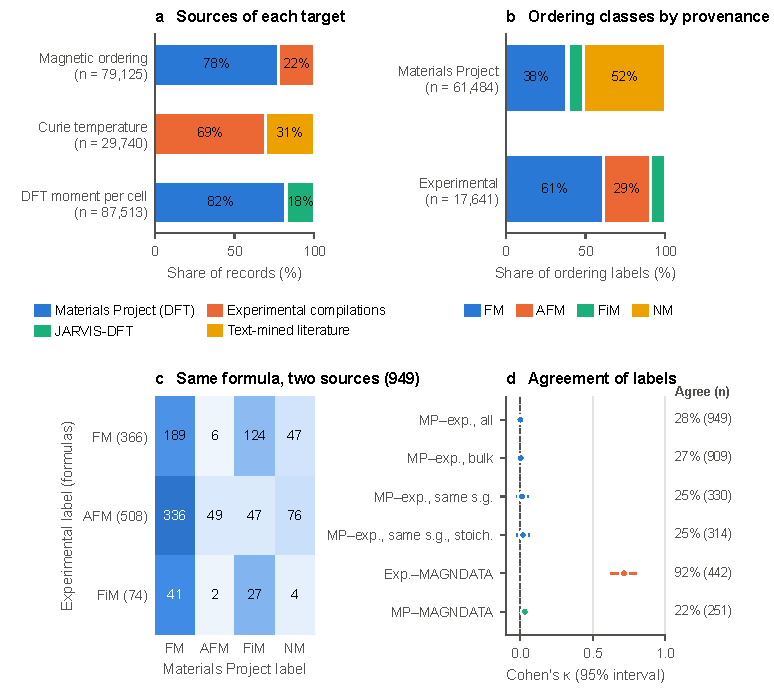
\includegraphics[width=\textwidth]{fig1.pdf}
\caption{\textbf{Non-magnetic DFT descriptors add little beyond composition.} Change in test performance from Tier~1 (composition) to Tier~2 (oxidation states) and to Tier~3 (non-magnetic DFT descriptors) on identical matched materials; positive values are improvements. Points are means over ten prespecified formula-grouped splits and bars are 95\% intervals that account for refitting (Nadeau--Bengio). \textbf{a}, Macro-F1 for magnetic ordering. \textbf{b}, MAE for the Curie temperature; ridge regression uses clipped inputs. \textbf{c}, MAE for the DFT moment per cell. \textbf{d}, MAE for the DFT moment per formula unit, including the effect of Tier~3 beyond a single site-count descriptor (grey). XGBoost values in \textbf{b} and \textbf{c} are means of eight realizations; those in \textbf{a} and \textbf{d} come from one.}\label{fig:rq1}
\end{figure}

\begin{figure}[p]
\centering
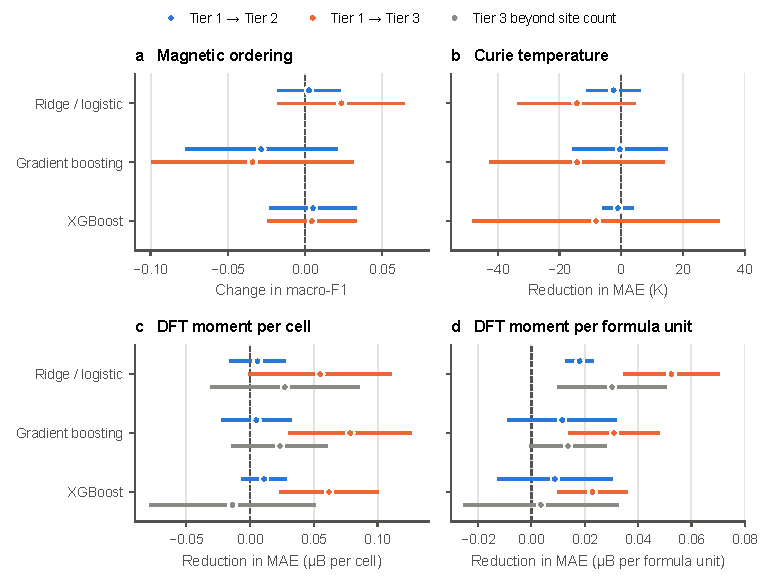
\includegraphics[width=\textwidth]{fig2.pdf}
\caption{\textbf{Average coverage hides subgroup failures.} \textbf{a},\textbf{b}, Coverage of 90\% prediction intervals for the Curie temperature (\textbf{a}) and the DFT moment per cell (\textbf{b}) under split, normalized and quantile (CQR) conformal prediction, for all test materials (blue) and for the highest predictions (orange; top decile in \textbf{a}, top third in \textbf{b}). Points are means over ten prespecified splits and bars are $\pm1$ s.d.\ across splits; in \textbf{b} most bars are smaller than the symbols. \textbf{c}, Mean coverage over the same splits of 90\% prediction sets for each ordering class (FM, ferromagnet; NM, non-magnet; AFM, antiferromagnet; FiM, ferrimagnet), for marginal and class-conditional sets. Dashed lines mark the nominal coverage.}\label{fig:rq2}
\end{figure}

\begin{figure}[p]
\centering
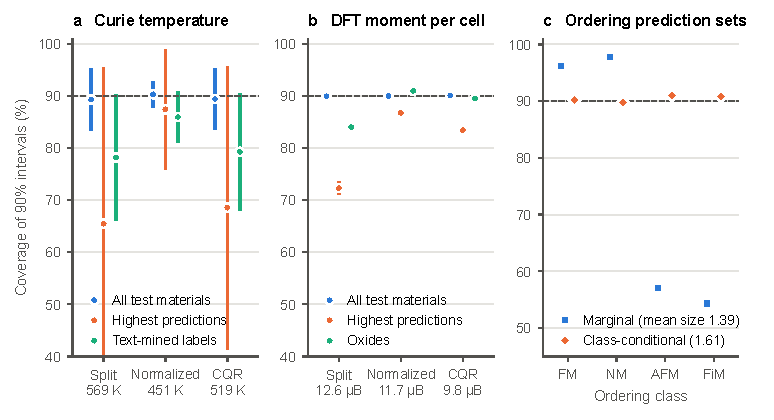
\includegraphics[width=\textwidth]{fig3.pdf}
\caption{\textbf{External benchmark of experimental Curie temperatures.} MAE (\textbf{a}) and $R^2$ (\textbf{b}) for nested novelty subsets of the external table, before (blue) and after (orange) the audit; the number of records after the audit is given in parentheses. `Blind', the composition never occurs in the training repository; `new paper', no source DOI was used in training; `unseen system', the set of elements never occurs in training. Points are estimates and bars are 95\% percentile intervals from a bootstrap over clusters of source papers (10,000 resamples); the bias-corrected intervals quoted in the text are in Extended Data Table~\ref{tab:ed_external}. Arrows mark lower limits of $R^2$ below $-1.5$.}\label{fig:rq3}
\end{figure}

\begin{figure}[p]
\centering
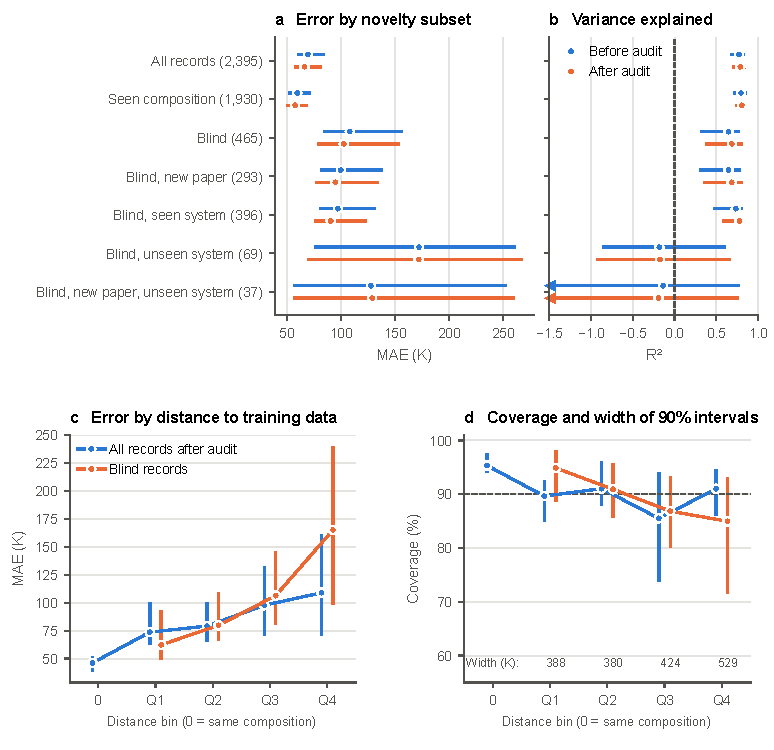
\includegraphics[width=\textwidth]{fig4.pdf}
\caption{\textbf{Error grows and coverage falls with distance from the training chemistry.} External records binned by composition distance to the nearest training formula (bin 0, identical composition; Q1--Q4, quartiles of the non-zero distances from closest to farthest), for all records after the audit and for the 465 blind records, which have no bin 0. \textbf{a}, MAE. \textbf{b}, Mean width of the 90\% normalized conformal interval. \textbf{c}, Coverage of that interval; the dashed line marks the nominal coverage. Bars are 95\% percentile intervals from a bootstrap over clusters of source papers.}\label{fig:distance}
\end{figure}

%% ===================================================================================================================
%% Extended Data (Nature Portfolio heading). Items are numbered Extended Data Fig. 1 and Extended Data Tables 1-7.
\clearpage
\begin{appendices}
\renewcommand{\figurename}{Extended Data Fig.}%
\renewcommand{\tablename}{Extended Data Table}%
\renewcommand{\thefigure}{\arabic{figure}}%
\renewcommand{\thetable}{\arabic{table}}%
\renewcommand{\theHfigure}{ED\arabic{figure}}%
\renewcommand{\theHtable}{ED\arabic{table}}%

\section{Extended Data}\label{sec:ed}

\begin{figure}[h]
\centering
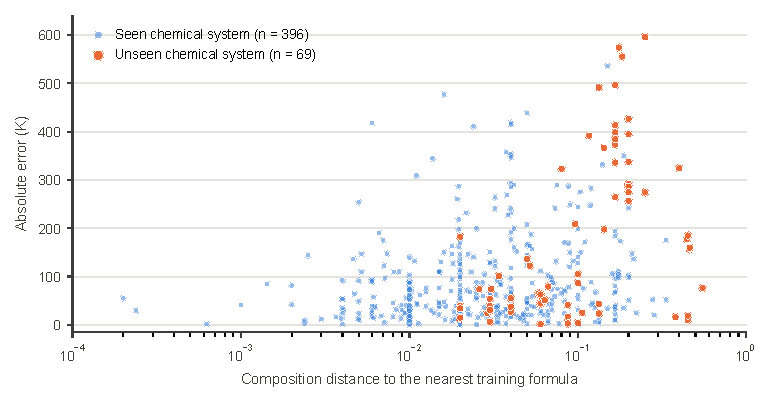
\includegraphics[width=\textwidth]{edfig1.pdf}
\caption{\textbf{Error against chemical distance for every blind external record.} Absolute error of the predicted Curie temperature against the composition distance to the nearest training formula (logarithmic axis) for the 465 blind records of the external benchmark, coloured by whether their chemical system occurs in the training data.}\label{fig:ed_scatter}
\end{figure}

\begin{table}[h]
\caption{\textbf{Effect of oxidation-state (Tier~2) and DFT (Tier~3) descriptors on matched populations.}}\label{tab:ed_tiers}%
\setlength{\tabcolsep}{2.5pt}%
\begin{tabular*}{\textwidth}{@{\extracolsep\fill}lllll@{}}
\toprule
Algorithm & Tier 1 $\to$ 2 & Tier 1 $\to$ 3 & \hd{Verdict\\(1 $\to$ 3)} & \hd{Holm\\$P$} \\
\midrule
\multicolumn{5}{@{}l}{\textit{Ordering, macro-F1}}\\
Ridge / logistic & $+0.003$ \ci{$-0.018$}{$+0.023$} & $+0.024$ \ci{$-0.018$}{$+0.065$} & none & 1.000 \\
Gradient boosting & $-0.028$ \ci{$-0.078$}{$+0.021$} & $-0.034$ \ci{$-0.100$}{$+0.032$} & none & 1.000 \\
XGBoost & $+0.005$ \ci{$-0.023$}{$+0.033$} & $+0.004$ \ci{$-0.024$}{$+0.033$} & none & 1.000 \\
Pooled (three algorithms) & -- & $-0.002$ \ci{$-0.035$}{$+0.031$} & none & -- \\
\midrule
\multicolumn{5}{@{}l}{\textit{Curie temperature, MAE (K)}}\\
Ridge (clipped) & $-2.5$ \ci{$-11.1$}{$+6.2$} & $-14.4$ \ci{$-33.5$}{$+4.8$} & none & -- \\
Gradient boosting & $-0.4$ \ci{$-15.7$}{$+14.9$} & $-14.3$ \ci{$-42.5$}{$+13.9$} & none & 1.000 \\
Boosting, larger search & -- & $-11.8$ \ci{$-35.2$}{$+11.7$} & borderline loss & -- \\
XGBoost & $-1.0$ \ci{$-6.0$}{$+3.9$} & $-8.2$ \ci{$-48.3$}{$+32.0$} & none & 1.000 \\
Pooled (three algorithms) & -- & $-12.3$ \ci{$-32.7$}{$+8.1$} & none & -- \\
\midrule
\multicolumn{5}{@{}l}{\textit{DFT moment per cell, MAE (\muB{} per cell)}}\\
Ridge / logistic & $+0.006$ \ci{$-0.016$}{$+0.028$} & $+0.055$ \ci{$-0.001$}{$+0.111$} & none & 0.373 \\
Gradient boosting & $+0.005$ \ci{$-0.023$}{$+0.033$} & $+0.079$ \ci{$+0.030$}{$+0.127$} & stable gain & 0.046 \\
XGBoost & $+0.011$ \ci{$-0.007$}{$+0.029$} & $+0.062$ \ci{$+0.023$}{$+0.101$} & stable gain & 0.046 \\
Pooled (three algorithms) & -- & $+0.065$ \ci{$+0.038$}{$+0.092$} & stable gain & -- \\
\midrule
\multicolumn{5}{@{}l}{\textit{DFT moment per formula unit, MAE (\muB{} per formula unit)}}\\
Ridge / logistic & $+0.018$ \ci{$+0.013$}{$+0.023$} & $+0.053$ \ci{$+0.035$}{$+0.070$} & stable gain & -- \\
Gradient boosting & $+0.012$ \ci{$-0.009$}{$+0.032$} & $+0.031$ \ci{$+0.014$}{$+0.048$} & stable gain & -- \\
XGBoost & $+0.009$ \ci{$-0.013$}{$+0.030$} & $+0.023$ \ci{$+0.010$}{$+0.036$} & stable gain & -- \\
\botrule
\end{tabular*}
\footnotetext{Improvement = deeper tier minus Tier~1 performance; positive = better. Identical matched rows, splits, grids and metrics at every tier; ten prespecified formula-grouped splits. Brackets: Nadeau--Bengio corrected resampled-$t$ 95\% intervals (refit-aware). Stable = this interval and the pooled formula-bootstrap interval both exclude zero and at least 7 of 10 splits share the sign; borderline = only one of the two intervals excludes zero; none = no stable change. Holm $P$: adjusted over the primary family of nine Tier~1 $\to$ 3 contrasts (ordering, Curie temperature and moment per cell, three algorithms each). The Curie ridge member of that family is the unclipped contrast (adjusted $P$ = 1.000; unclipped ridge is numerically unstable, $-825$~K); using the clipped contrast gives 0.740 and leaves the other eight unchanged. Ridge for the Curie temperature uses inputs clipped to the 1st and 99th percentiles of the training fold. XGBoost: mean of eight thread/seed realizations for the Curie temperature and the moment per cell, one realization otherwise. Pooled = in each split the mean of the three algorithms' improvements (clipped ridge for the Curie temperature); secondary and unadjusted; its minimum detectable effect is 28.4~K for the Curie temperature, 0.037~\muB{} per cell for the moment and 0.046 macro-F1 for ordering. Larger search: 64 candidate settings for gradient boosting instead of 4, secondary and unadjusted (minimum detectable effect 32.6~K); the formula-bootstrap interval is $-21.9$ to $-0.04$~K, which is why the verdict is a borderline loss. The gradient-boosting Tier~1 $\to$ 2 change for ordering is a borderline loss (the bootstrap interval excludes zero). Moment per formula unit: 10,821 rows; the effect of Tier~3 beyond a site-count descriptor is in Fig.~\ref{fig:rq1}d and Supplementary Table~8.}
\end{table}

\begin{table}[h]
\caption{\textbf{Magnetic and structure-aware physics for the Curie temperature.}}\label{tab:ed_magphys}%
\setlength{\tabcolsep}{4pt}%
\begin{tabular*}{\textwidth}{@{\extracolsep\fill}lrllll@{}}
\toprule
Algorithm & MAE (K) & vs Tier 1 & Verdict & vs Tier 3 & Verdict \\
\midrule
\multicolumn{6}{@{}l}{\textit{Tier 1 + magnetic-sublattice geometry (10 descriptors)}}\\
Gradient boosting & 202.6 & $+0.3$ \ci{$-13.9$}{$+14.5$} & none & -- & -- \\
XGBoost & 203.6 & $+5.8$ \ci{$-15.8$}{$+27.4$} & none & -- & -- \\
\midrule
\multicolumn{6}{@{}l}{\textit{Tier 3 + magnetic-sublattice geometry}}\\
Gradient boosting & 220.2 & -- & -- & $-3.1$ \ci{$-27.6$}{$+21.4$} & none \\
XGBoost & 211.0 & -- & -- & $+8.0$ \ci{$-15.8$}{$+31.9$} & none \\
\midrule
\multicolumn{6}{@{}l}{\textit{Tier 3 + DFT magnetic outputs (4 descriptors)}}\\
Gradient boosting & 197.6 & $+5.3$ \ci{$-29.9$}{$+40.4$} & none & $+19.6$ \ci{$-3.1$}{$+42.3$} & borderline \\
XGBoost & 210.7 & $-1.4$ \ci{$-35.8$}{$+33.0$} & none & $+8.3$ \ci{$-27.5$}{$+44.2$} & none \\
\midrule
\multicolumn{6}{@{}l}{\textit{Tier 3 + geometry + DFT magnetic outputs}}\\
Gradient boosting & 205.6 & $-2.8$ \ci{$-39.1$}{$+33.6$} & none & $+11.5$ \ci{$-14.4$}{$+37.4$} & none \\
XGBoost & 201.9 & $+7.5$ \ci{$-33.8$}{$+48.8$} & none & $+17.2$ \ci{$-9.5$}{$+43.9$} & borderline \\
\midrule
\multicolumn{6}{@{}l}{\textit{Tier 3 + CHGNet crystal embedding (64 dimensions)}}\\
Gradient boosting & 213.7 & $-10.8$ \ci{$-22.5$}{$+0.9$} & none & $+3.5$ \ci{$-19.2$}{$+26.2$} & none \\
XGBoost & 199.9 & $+9.5$ \ci{$-28.7$}{$+47.7$} & none & $+19.2$ \ci{$+0.4$}{$+38.0$} & stable \\
\botrule
\end{tabular*}
\footnotetext{Matched Curie population (4,602 records) and the same ten splits as Extended Data Table~\ref{tab:ed_tiers}. MAE of Tier~1 and Tier~3: gradient boosting 202.9 and 217.1~K, XGBoost 209.3 and 219.1~K. Improvements in K, positive = better, with Nadeau--Bengio 95\% intervals; verdicts refer to gains and are defined as in Extended Data Table~\ref{tab:ed_tiers}. Geometry: magnetic-ion site fraction and density, nearest and mean M--M distance, M--M connectivity, M--X distance and coordination, mean M--X--M angle and the fractions of angles in 150--180$^\circ$ and 80--100$^\circ$, from the Materials Project structure of the same entry. DFT magnetic outputs (moment per atom, magnetic-site fraction, magnetization per volume, magnetic flag) cannot leak experimental Curie temperatures. CHGNet: frozen 64-dimensional crystal feature of the pretrained universal potential. XGBoost: one realization.}
\end{table}

\begin{table}[h]
\caption{\textbf{Coverage of 90\% conformal prediction intervals, overall and in subgroups.}}\label{tab:ed_intervals}%
\setlength{\tabcolsep}{4pt}%
\begin{tabular*}{\textwidth}{@{\extracolsep\fill}lrrrrr@{}}
\toprule
Method & \hd{All test materials,\\mean (s.d.)} & \hd{Mean\\width} & \hd{Highest\\predictions} & \hd{Second\\subgroup} & \hd{Farthest\\distance decile} \\
\midrule
\multicolumn{6}{@{}l}{\textit{Curie temperature (highest: top decile; second: text-mined labels)}}\\
Split conformal & 89.3 (6.0) & 569 K & 65.5 & 78.2 & 86.6 \\
Normalized conformal & 90.3 (2.5) & 451 K & 87.4 & 86.0 & 88.2 \\
CQR & 89.4 (5.8) & 519 K & 68.6 & 79.3 & 89.7 \\
\midrule
\multicolumn{6}{@{}l}{\textit{DFT moment per cell (highest: top third; second: oxides)}}\\
Split conformal & 90.0 (0.4) & 12.6 \muB{} & 72.3 & 84.0 & -- \\
Normalized conformal & 90.0 (0.5) & 11.7 \muB{} & 86.7 & 91.0 & -- \\
CQR & 90.1 (0.4) & 9.8 \muB{} & 83.4 & 89.5 & -- \\
\botrule
\end{tabular*}
\footnotetext{Coverage in \%; nominal 90\%; ten prespecified formula-grouped splits; calibration on 20\% of the training formulas. Subgroups are defined without the difficulty score of any method: the highest point predictions, the text-mined label source (Curie temperature) or oxides (moment), and the farthest decile of composition distance to the training formulas. For comparison, on the decile defined by the normalized method's own difficulty scale (a circular definition used in an earlier analysis), Curie coverage was 54, 89 and 61\% for split, normalized and CQR. Every Curie subgroup that we evaluated is in Supplementary Table~11.}
\end{table}

\begin{table}[h]
\caption{\textbf{Calibration of magnetic-ordering probabilities and prediction sets.}}\label{tab:ed_ordcal}%
\setlength{\tabcolsep}{4pt}%
\begin{tabular*}{\textwidth}{@{\extracolsep\fill}lrrrrrrrr@{}}
\toprule
& \multicolumn{2}{c}{ECE} & \multicolumn{5}{c}{Coverage (\%)} & \\
\cmidrule{2-3}\cmidrule{4-8}
Probabilities or sets & \hd{Top\\label} & \hd{Class-\\wise} & All & FM & AFM & FiM & NM & \hd{Set\\size} \\
\midrule
Raw (balanced weights) & 0.064 & 0.035 & -- & -- & -- & -- & -- & -- \\
Prior-corrected & 0.090 & 0.049 & -- & -- & -- & -- & -- & -- \\
Prior-corrected + temperature & 0.014 & 0.032 & -- & -- & -- & -- & -- & -- \\
Marginal sets & -- & -- & 89.8 & 96.2 & 57.0 & 54.3 & 97.7 & 1.39 \\
Class-conditional sets & -- & -- & 90.1 & 90.1 & 90.9 & 90.8 & 89.8 & 1.61 \\
\botrule
\end{tabular*}
\footnotetext{Means over ten prespecified splits (Tier~1 XGBoost, full ordering population). ECE, expected calibration error with 15 equal-width bins. Sets are at 90\% nominal coverage on prior-corrected, temperature-scaled probabilities; the temperature was fitted on half of the calibration formulas and the conformal thresholds on the other half (re-using one calibration set changes coverage by less than 0.3 points). Standard deviation of overall coverage across splits: 0.9 (marginal) and 0.6 (class-conditional) points.}
\end{table}

\begin{table}[h]
\caption{\textbf{Generalization to unfamiliar chemical systems and to another label source.}}\label{tab:ed_general}%
\setlength{\tabcolsep}{4pt}%
\begin{tabular*}{\textwidth}{@{\extracolsep\fill}llrrlr@{}}
\toprule
Test & Metric & Familiar & Unfamiliar & \hd{Change or 95\%\\interval} & \hd{Splits worse\\or null limit} \\
\midrule
\multicolumn{6}{@{}l}{\textit{Leave chemical system out (ten paired splits)}}\\
Ordering & macro-F1 & 0.712 & 0.684 & $-0.028$ \ci{$-0.041$}{$-0.016$} & 10/10 \\
Curie temperature & MAE (K) & 99.2 & 101.9 & $+2.7$ \ci{$-16.8$}{$+22.2$} & 5/10 \\
DFT moment per cell & MAE (\muB{}) & 2.591 & 2.663 & $+0.073$ \ci{$-0.009$}{$+0.154$} & 7/10 \\
\midrule
\multicolumn{6}{@{}l}{\textit{Label source, ordering on FM, AFM and FiM (metric: balanced accuracy)}}\\
MP $\to$ experimental & -- & 0.769 & 0.337 & \ci{0.273}{0.396} & 0.374 \\
Experimental $\to$ MP & -- & 0.591 & 0.384 & \ci{0.366}{0.401} & 0.351 \\
\botrule
\end{tabular*}
\footnotetext{Leave chemical system out: the formula-grouped and system-grouped test sets differ, so each change combines novelty with test-set composition; change = unfamiliar minus familiar with a 95\% interval; last column, splits (of ten) in which the unfamiliar setting was worse. Label source (MP, Materials Project): `familiar' = a model trained and tested within the target label source, `unfamiliar' = trained on the other source; last column, 97.5th percentile of the null distribution; NM removed on both sides (the experimental labels contain 5 NM rows); training formulas present in the target test set removed; 95\% formula-bootstrap interval of the unfamiliar value; null = 20 refits on permuted training labels. Label agreement for the 949 formulas labelled by both sources: 28\%, Cohen's $\kappa$ = 0.00 \ci{$-0.03$}{0.03} (Supplementary Table~12).}
\end{table}

\begin{table}[h]
\caption{\textbf{External experimental Curie benchmark by novelty subset.}}\label{tab:ed_external}%
\setlength{\tabcolsep}{3pt}%
\begin{tabular*}{\textwidth}{@{\extracolsep\fill}lrlllr@{}}
\toprule
Subset & $n$ (clusters) & MAE (K) & $R^2$ & Skill & Coverage \\
\midrule
All records & 2,395 (464) & \est{66.5}{57.2}{81.1} & \est{0.79}{0.69}{0.85} & \est{0.80}{0.70}{0.85} & 0.925 \\[1pt]
Seen composition & 1,930 (440) & \est{57.7}{50.7}{70.4} & \est{0.80}{0.72}{0.86} & \est{0.83}{0.74}{0.87} & 0.933 \\[1pt]
\quad seen, value not copied & 767 (208) & \est{84.5}{68.1}{110.2} & \est{0.70}{0.53}{0.80} & \est{0.71}{0.53}{0.81} & 0.890 \\[1pt]
Blind & 465 (81) & \est{102.7}{75.1}{143.6} & \est{0.69}{0.43}{0.82} & \est{0.70}{0.41}{0.84} & 0.895 \\[1pt]
\quad new paper & 293 (61) & \est{95.1}{73.1}{125.7} & \est{0.68}{0.43}{0.83} & \est{0.72}{0.50}{0.86} & 0.898 \\[1pt]
\quad seen system & 396 (72) & \est{90.6}{71.8}{116.0} & \est{0.78}{0.67}{0.87} & \est{0.79}{0.66}{0.89} & 0.902 \\[1pt]
\quad unseen system & 69 (18) & \est{171.9}{82.6}{293.7} & \est{$-0.17$}{$-1.02$}{0.64} & \est{$-0.17$}{$-0.77$}{0.56} & 0.855 \\[1pt]
\quad new paper, unseen system & 37 (12) & \est{129.0}{61.8}{297.0} & \est{$-0.19$}{$-6.17$}{0.70} & \est{0.04}{$-1.03$}{0.69} & 0.757 \\
\botrule
\end{tabular*}
\footnotetext{Primary benchmark after the audit (2,395 of 2,500 records). Seen or blind by composition identity; `new paper', no source DOI used in training; `unseen system', the set of elements never occurs in training. Clusters: source-paper components (records linked by any shared DOI), the resampling unit; 95\% BCa cluster-bootstrap intervals (10,000 resamples). Skill = 1 $-$ MSE/MSE of a constant prediction equal to the training mean (338~K), a fixed reference for all subsets. Coverage of the 90\% normalized conformal interval. Results under first-DOI and chemical-system clustering are in Supplementary Table~4.}
\end{table}

\begin{table}[h]
\caption{\textbf{What the predictions support in a screening setting (465 blind external records).}}\label{tab:ed_screening}%
\setlength{\tabcolsep}{4pt}%
\begin{tabular*}{\textwidth}{@{\extracolsep\fill}lrlrl@{}}
\toprule
Rule & $n$ (papers) & Measure & Estimate & 95\% interval \\
\midrule
\multicolumn{5}{@{}l}{\textit{Abstention}}\\
No abstention & 465 (81) & MAE (K) & 103 & \ci{78}{154} \\
 & & coverage & 0.89 & \ci{0.83}{0.92} \\
Keep the 50\% closest compositions & 238 (42) & MAE (K) & 71 & \ci{61}{97} \\
 & & coverage & 0.93 & \ci{0.88}{0.96} \\
Keep the 50\% narrowest intervals & 233 (50) & MAE (K) & 73 & \ci{59}{109} \\
 & & coverage & 0.88 & \ci{0.77}{0.92} \\
\midrule
\multicolumn{5}{@{}l}{\textit{Room-temperature screen (\Tc{} $>$ 300 K)}}\\
Point prediction & 465 (81) & accuracy & 0.802 & \ci{0.717}{0.879} \\
 & & recall & 0.936 & \ci{0.866}{0.973} \\
 & & precision & 0.769 & \ci{0.667}{0.902} \\
Decide only if the 90\% interval & 465 (81) & share decided & 0.374 & \ci{0.261}{0.598} \\
\quad excludes 300 K & & accuracy of decisions & 0.925 & \ci{0.837}{0.982} \\
\botrule
\end{tabular*}
\footnotetext{The 465 blind external records; base rate of \Tc{} $>$ 300~K = 0.57. Paper-cluster bootstrap 95\% intervals (10,000 resamples). Distance: composition (total-variation) distance to the nearest training formula; interval: the 90\% normalized conformal interval.}
\end{table}

\begin{table}[h]
\caption{\textbf{Screening rules on the internal test sets (Curie temperature, ten splits).}}\label{tab:ed_internal}%
\setlength{\tabcolsep}{4pt}%
\begin{tabular*}{\textwidth}{@{\extracolsep\fill}lrrr@{}}
\toprule
Rule & \hd{Retained\\share} & MAE (K) & Coverage \\
\midrule
\multicolumn{4}{@{}l}{\textit{Abstention}}\\
No abstention & 1.000 & 102.9 (19.1) & 0.903 (0.025) \\
Keep the narrowest intervals & 0.761 & 62.5 (5.9) & 0.912 (0.016) \\
 & 0.500 & 42.5 (4.1) & 0.920 (0.015) \\
 & 0.250 & 30.8 (2.6) & 0.920 (0.020) \\
Keep the closest compositions & 0.757 & 100.1 (26.2) & 0.910 (0.030) \\
 & 0.508 & 85.6 (28.6) & 0.919 (0.036) \\
 & 0.271 & 103.0 (58.8) & 0.914 (0.063) \\
\midrule
\multicolumn{4}{@{}l}{\textit{Room-temperature screen (\Tc{} $>$ 300 K; base rate 0.454 (0.020))}}\\
Point prediction: accuracy & & & 0.857 (0.018) \\
\quad precision & & & 0.822 (0.042) \\
\quad recall & & & 0.876 (0.028) \\
Interval decisions: share decided & & & 0.437 (0.043) \\
\quad accuracy of decisions & & & 0.976 (0.015) \\
Precision among the 25 highest predictions & & & 0.956 (0.126) \\
\quad 50 highest & & & 0.952 (0.119) \\
\quad 100 highest & & & 0.921 (0.126) \\
\botrule
\end{tabular*}
\footnotetext{Mean (standard deviation across splits) over the ten prespecified formula-grouped splits, about 4,460 test rows each; Tier~1 XGBoost and 90\% normalized conformal intervals from the uncertainty runs, whose ten splits and 80\% training share differ from the frozen split (MAE 76~K for the baseline in Results). The standard deviation is descriptive because the test sets of different splits overlap. Ties at a distance cut-off are kept, so the retained share can exceed the nominal 0.75, 0.50 and 0.25. Interval decisions: a record is decided only if its 90\% interval lies wholly above or wholly below 300 K. Rules and thresholds as for the external records (Extended Data Table~\ref{tab:ed_screening}).}
\end{table}

\end{appendices}

\end{document}
